
%%%%%%%%%%%%%%%%%%%%%%%%%%%%%%%%%%%%%%%%%%%%%%%%%%
% Basic setup. Most papers should leave these options alone.
\documentclass[fleqn,usenatbib]{mnras}

\usepackage[T1]{fontenc}
\DeclareRobustCommand{\VAN}[3]{#2}
\let\VANthebibliography\thebibliography
\def\thebibliography{\DeclareRobustCommand{\VAN}[3]{##3}\VANthebibliography}

%%%%% AUTHORS - PLACE YOUR OWN PACKAGES HERE %%%%%
\usepackage{graphicx}	% Including figure files
\usepackage{amsmath}	% Advanced maths commands
\usepackage{amssymb}	% Extra maths symbols
\usepackage{xspace} 
\usepackage{xcolor}
\usepackage{upgreek}
\usepackage{CJK}
\usepackage{fontawesome}
\usepackage{gensymb}
\usepackage{multirow}
\usepackage{mathtools}
\usepackage{newtxtext,newtxmath}
\usepackage{tabularx}

%%%%% AUTHORS - PLACE YOUR OWN COMMANDS HERE %%%%%
\newcommand{\ToDo}[1]{\textbf{\textcolor{blue}{ToDo: #1}}}
\newcommand{\SB}[1]{{\textcolor{purple}{SB: #1}}}
\newcommand{\TB}[1]{{\textcolor{blue}{TB: #1}}}
\newcommand{\Gaia}{\textit{Gaia}\xspace} % \Gaia
\newcolumntype{C}{>{\centering\arraybackslash}X}

%%%%%%%%%%%%%%%%%%%%%%%%%%%%%%%%%%%%%%%%%%%%%%%%%%
%%%%%%%%%%%%%%%%%%% TITLE PAGE %%%%%%%%%%%%%%%%%%%

% Title of the paper, and the short title which is used in the headers.
% Keep the title short and informative.
\title[Radial metallicity gradients in NIHAO]{More than just a line: Shining light on the flattening radial metallicity gradient of a NIHAO Milky-Way analogue simulation}

% The list of authors, and the short list which is used in the headers.
% If you need two or more lines of authors, add an extra line using \newauthor
\author[S. Buder and T. Buck]{
S. Buder,$^{1,2}$\thanks{E-mail: sven.buder@anu.edu.au} and
T. Buck,$^{3,4}$
\\
% List of institutions
$^{1}$Research School of Astronomy \& Astrophysics, Australian National University, ACT 2611, Australia\\
$^{2}$Center of Excellence for Astrophysics in Three Dimensions (ASTRO-3D), Australia\\
$^{3}$Universit{\"a}t Heidelberg, Interdisziplin{\"a}res Zentrum f{\"u}r Wissenschaftliches Rechnen, Im Neuenheimer Feld 205, D-69120 Heidelberg, Germany\\
$^{4}$Universit{\"a}t Heidelberg, Zentrum f{\"u}r Astronomie, Institut f{\"u}r Theoretische Astrophysik, Albert-Ueberle-Straße 2, D-69120 Heidelberg, Germany
}

% These dates will be filled out by the publisher
\date{Accepted YYYY Month DD. Received YYYY Month DD}

% Enter the current year, for the copyright statements etc.
\pubyear{2024}

% Don't change these lines
\begin{document}
\label{firstpage}
\pagerange{\pageref{firstpage}--\pageref{lastpage}}
\maketitle

% Abstract of the paper
\begin{abstract} % XXX words
% Context
Radial metallicity gradients in galaxies are crucial for understanding the processes of galactic formation and its dynamical and chemical evolution.
% Method
We use young stars and gas of a high-resolution simulation of a NIHAO Milky Way analogue galaxy to analyse four properties of the radial metallicity gradient, namely its linearity and scatter as well as its coherence with radial coverage, azimuth, and age.
% Results
While a global linear fit with slope traces the gradient well, we find it to be too flat in the inner galaxy and too steep in the outer galaxy. An initially stepper but then flattening second order quadratic function provides a superior fit down to the smallest radial steps, where less regular effects take over. We identify these as \SB{spiral arms or warp?} when tracing them across the Galactic position. The simulation further exhibits a steadily increasing spread in [Fe/H] even among the young stars from 0.01 dex in the inner galaxy to 0.14 dex in at a radius 20 kpc coinciding with decreasing stellar density and increased flaring of stars towards higher heights with little correlation across the small age range of 1 Gyr.
% Conculsions
We conclude that future Galactic and extragalactic observational studies should test our theoretical prediction of a quadratic gradient function with their data to confirm or reject previous observational claims of a broken linear radial metallicity gradients proposed for the Milky Way and other spiral galaxies, as either function implies different dynamical and chemical galaxy formation and evolution scenarios.
\end{abstract}
% Select between one and six entries from the list of approved keywords.
% Don't make up new ones.
\begin{keywords}
cosmology: observations -- Galaxy: structure -- Galaxy: abundances  -- galaxies: structure -- galaxies: abundances
\end{keywords}

%%%%%%%%%%%%%%%%%%%%%%%%%%%%%%%%%%%%%%%%%%%%%%%%%%

%%%%%%%%%%%%%%%%% BODY OF PAPER %%%%%%%%%%%%%%%%%%

\section{Introduction}
\label{sec:intro}

Radial metallicity gradients in galaxies, defined as the change in metal abundance with galactocentric radius, offer vital insights into the processes that shape the chemical and dynamical evolution of galaxies. The decrease in metallicity with increasing distance from the Galactic center is well-established both theoretically \citep{Larson1976, Tinsley1980, Chiosi1980} and observationally in the Milky Way \citep{Searle1971, Janes1979, Twarog1997}. However, the specific shape and characteristics of this gradient remain somewhat unclear.

The Milky Way, being the only galaxy where we can resolve millions of stars, provides a unique opportunity to study these gradients in detail. Over two decades ago, \citet{Chiappini2002} highlighted the contradictions in the observed shape, magnitude, and evolution of abundance gradients. Recent advancements, such as the \textit{Gaia} mission \citep{Gaia-Collaboration2016}, have significantly expanded our observational data, allowing for more detailed studies of these gradients.

For instance, \citet{Hogg2019} created an extensive metallicity map of the Milky Way using APOGEE and \textit{Gaia} data, while \citet{Poggio2022} mapped young stars and found a metallicity excess around spiral arms \citep[see also][]{Zari2018, Zari2021, Poggio2021, Hackshaw2024}. Similarly, \citet[][among others]{Imig2023} traced gradients across different stellar populations and ages, emphasizing the importance of considering radial migration effects \citep{Binney2008, Frankel2018, Frankel2020}.

Historically, radial metallicity gradients have been measured using various stellar populations and gas tracers. Early evidence by \citet{Janes1979} suggested a gradient on the order of
\begin{equation}
\frac{\mathrm{d{[Fe/H]}}}{\mathrm{d}R} = -0.05 \pm 0.01,\mathrm{dex,kpc^{-1}}
\end{equation}
for the Milky Way which aligns with more recent measurements \citep{Anders2017, Hayden2015}. Estimated gradients also seem to be broadly consistent across different stellar tracers, such as young open clusters \citep[e.g.][]{Cunha2016, Magrini2017, Casamiquela2019, Donor2020, Spina2021,Myers2022}, young hot (OB-type) stars \citep{Zari2018, Zari2021, Poggio2021, Poggio2022}, field stars close to the Galactic plane \citep[e.g.][]{Bergemann2014} or Cepheids \citep{Andrievsky2002, Andrievsky2002b, Lemasle2007, Lemasle2013}. However, these gradients are accompanied by significant spread in [Fe/H] of $0.1-0.15\,\mathrm{dex}$, as noted by \citet{Twarog1980}, which may imply a fine structure of the metallicity gradient \citep[see][]{Genovali2014}.

Despite extensive observational efforts, several challenges persist:
\begin{itemize}
    \item The completeness (or patchiness) of observed datasets remains a fundamental issue \citep{Bergemann2014}.
    \item How robustly can we use the incomplete data to predict substructure in the gradients, such as the need to actually fit two linear gradients with a break radius at corotation radius \citep[][and references therein]{Bresolin2012} or further out \citep{Donor2020} - or even more complicated functions \citep[see e.g.][]{Chiappini2001, Kubryk2015}?
    \item Different samples yield varying gradients, potentially due to biases in data or the inclusion of older stars \citep[e.g.][]{Boeche2013, AllendePrieto2006, Katz2011, Hayden2014, Anders2014, Vickers2021, Willett2023}.
    \item The impact of spiral arm structures \citep{Poggio2021}, the Galactic warp \citep{Lemasle2022} or bar-driven mixing \citep{DiMatteo2013} on metallicity gradients is not fully understood.
    \item Methodologies for fitting linear models to scattered data need re-evaluation \citep{Metha2021}.
\end{itemize}

Understanding these gradients in the Milky Way is also crucial for extragalactic studies, where spatial resolution limits observations. New instruments like the MUSE integral field spectrograph has enabled a plethora of extragalactic studies to contrast the Milky Way to and techniques like the spectroscopy of HII regions and planetary nebulae have helped to infer gas metallicity distributions in external galaxies \citep{Shaver1983, Vilchez1996, Rolleston2000, Bresolin2012}. Recent examples include \citet{Sanchez2014} with CALIFA galaxy observations as well as \citet{Mun2024} and \citet{Chen2024} who use MAGPI galaxy observations to probe for example the effects of spiral arms. Notable is also the scatter that \citet{Chen2023} found for the gas metallicity across galactic radius with TYPHOON observations (see their. Figs. 4-6).

From a modelling perspective, galactic chemical evolution models can both test understanding of radial metallicity gradients and make predictions beyond the limited volumes and tracers tested by Milky Way and extragalactic studies. Such galactic chemical evolution models include \citet{Chiappini2001, Minchev2014b, Kubryk2015, Stanghellini2015, Matteucci2001b}.

New suites of large-scale simulations now allow to gain insights into radial metallicity gradients across a range of simulated galaxies - including Milky Way analogues. While \citet{Pilkington2012} found that such gradients are established by inside-out formation in RaDES simulations, whereas \citet{Tissera2019} used EAGLE simulations to study gradients across different galaxy characteristics, such as mergers and stellar mass. \citet{Bellardini2021} and \citet{Bellardini2022, Graf2024} compared the radial metallicity gradient and its azimuthal scatter for different simulations of the FIRE suite for gas and stars, respectively. Focusing on the change of the radial metallicity gradient over time, \citet{Grand2015} assessed the scatter of radial metallicity distribution for different stellar ages. Both \citet[][see their Fig. 6]{Ma2017} with FIRE and \citet[see their Fig. 9][]{Agertz2021} with VINTERGATAN further assessed the evolution of the radial metallicity gradient for gas and stars. \citet{Khoperskov2023e} again focused on the gas and found the scatter of the gas metallicity of $\approx 0.04-0.06\,\mathrm{dex}$ at a given galactocentric distance.

This study aims to advance these theoretical insight by addressing four critical scientific questions using a high-resolution simulation of a Milky Way analogue galaxy:
\begin{enumerate}
\item \textit{Linearity of the gradient:} Assess the extent to which the radial metallicity gradient of young stars is linear.
\item \textit{Scatter in the gradient:} Quantify the expected scatter in the radial metallicity gradient of young stars.
\item \textit{Coherence of the gradient with position:} Investigate the gradient's variation with radial coverage and azimuth.
\item \textit{Coherence of the gradient with age:} Determine the reliability of stars as tracers of the gas disk over different ages.
\end{enumerate}

The paper is structured as follows: Section~\ref{sec:data} describes the data of our Milky Way analogue NIHAO simulation. Section~\ref{sec:radial_metallicity_gradients} analyses the radial metallicity gradients of the simulation under the four aforementioned questions. Section~\ref{sec:discussion} discusses them individually and Section~\ref{sec:conc} bundles them into an overarching conclusion.

\section{Data: A NIHAO Milky Way analogue simulation} \label{sec:data}

For this project, we use a cosmological zoom-in simulation of a Milky Way analogue (\texttt{g8.26e11}) from the \textit{Numerical Investigation of a Hundred Astronomical Objects} \citep[NIHAO,][]{Wang2015}. The model volume has a total mass (gas, stars and dark matter) of $8.26 \cdot 10^{11}\,\mathrm{M_\odot}$ and contains $4 \cdot 10^{10}\,\mathrm{M_\odot}$ stellar mass with a stellar mass resolution of $1.06 \cdot 10^{5}\,\mathrm{M_\odot}$ \citep{Buck2021} and was calculated as part of the NIHAO-UHD project \citep{Buck2020b}.

Simulations were carried out with the smoothed particle hydrodynamics code \texttt{Gasoline2} \citep{Wadsley2017} using cosmological parameters from \citet{Planck2014} with initial conditions and energetic feedback descriptions from the NIHAO project \citep{Wang2015}. Zoom-in simulations were then performed as described in detail by \citet{Buck2021} with star formation following \citet{Stinson2006} and energetic feedback following \citet{Stinson2013}.

Because computational resources still limit the mass resolution of simulations, we are relying on tracer particles that represent simple stellar populations (SSPs) with the same age, overall metallicity and discrete initial mass function (IMF). \citet{Buck2021} have implemented the flexible chemical evolution code \textsc{chempy} \citep{Rybizki2017} to calculate the chemical yields for the SSPs. In particular, we use the alternative (\texttt{alt}) setup of \textsc{chempy} that assumes a \citet{Chabrier2003} IMF with high-mass slope of $\alpha_\text{IMF} = -2.3$ over a mass range of $0.1-100\,\mathrm{M_\odot}$ for SSPs across a metallicity range of $Z/Z_\odot \in [10^{-5},2]$. The code calculates the contribution from asymptotic giant branch (AGB) stars, CCSN across a mass range of $8-40\,\mathrm{M_\odot}$, and SNIa with a an exponential function with exponent $-1.12$, a delay time of $40\,\mathrm{Myr}$, and a normalization of the SNI rate of -2.9. For each of these nucleosynthetic channels, yields from the following studies are used: \citet{Limongi2018} for CCSN, \citet{Seitenzahl2013} for SNIa, and \citet{Karakas2016} for AGB stars. Contrary to a previous study by \citet{Buder2024}, we take the elemental abundances at face value and do not apply any shifts.

For this project, we limit the simulation data to the main halo by applying \textsc{pynbody}'s implementation of the Amiga Halo Finder \citep{Knollman2009} and then reposition and rotate this main halo to be face-on based on the angular momentum with \textsc{pynbody}'s \textsc{analysis.angmom.faceon} module \citep{pynbody}. The main halo has a total half mass radius of $66.0\,\mathrm{kpc}$ for all matter and a stellar half mass radius $2.4\,\mathrm{kpc}$. We then further transform the resulting galactocentric Cartesian coordinate $(X,Y,Z)$ and velocities $(V_X,V_Y,V_Z)$ to Cylindrical ones as done in a previous study of this main halo by \citet{Buder2024}.

\begin{figure*}
    \centering
    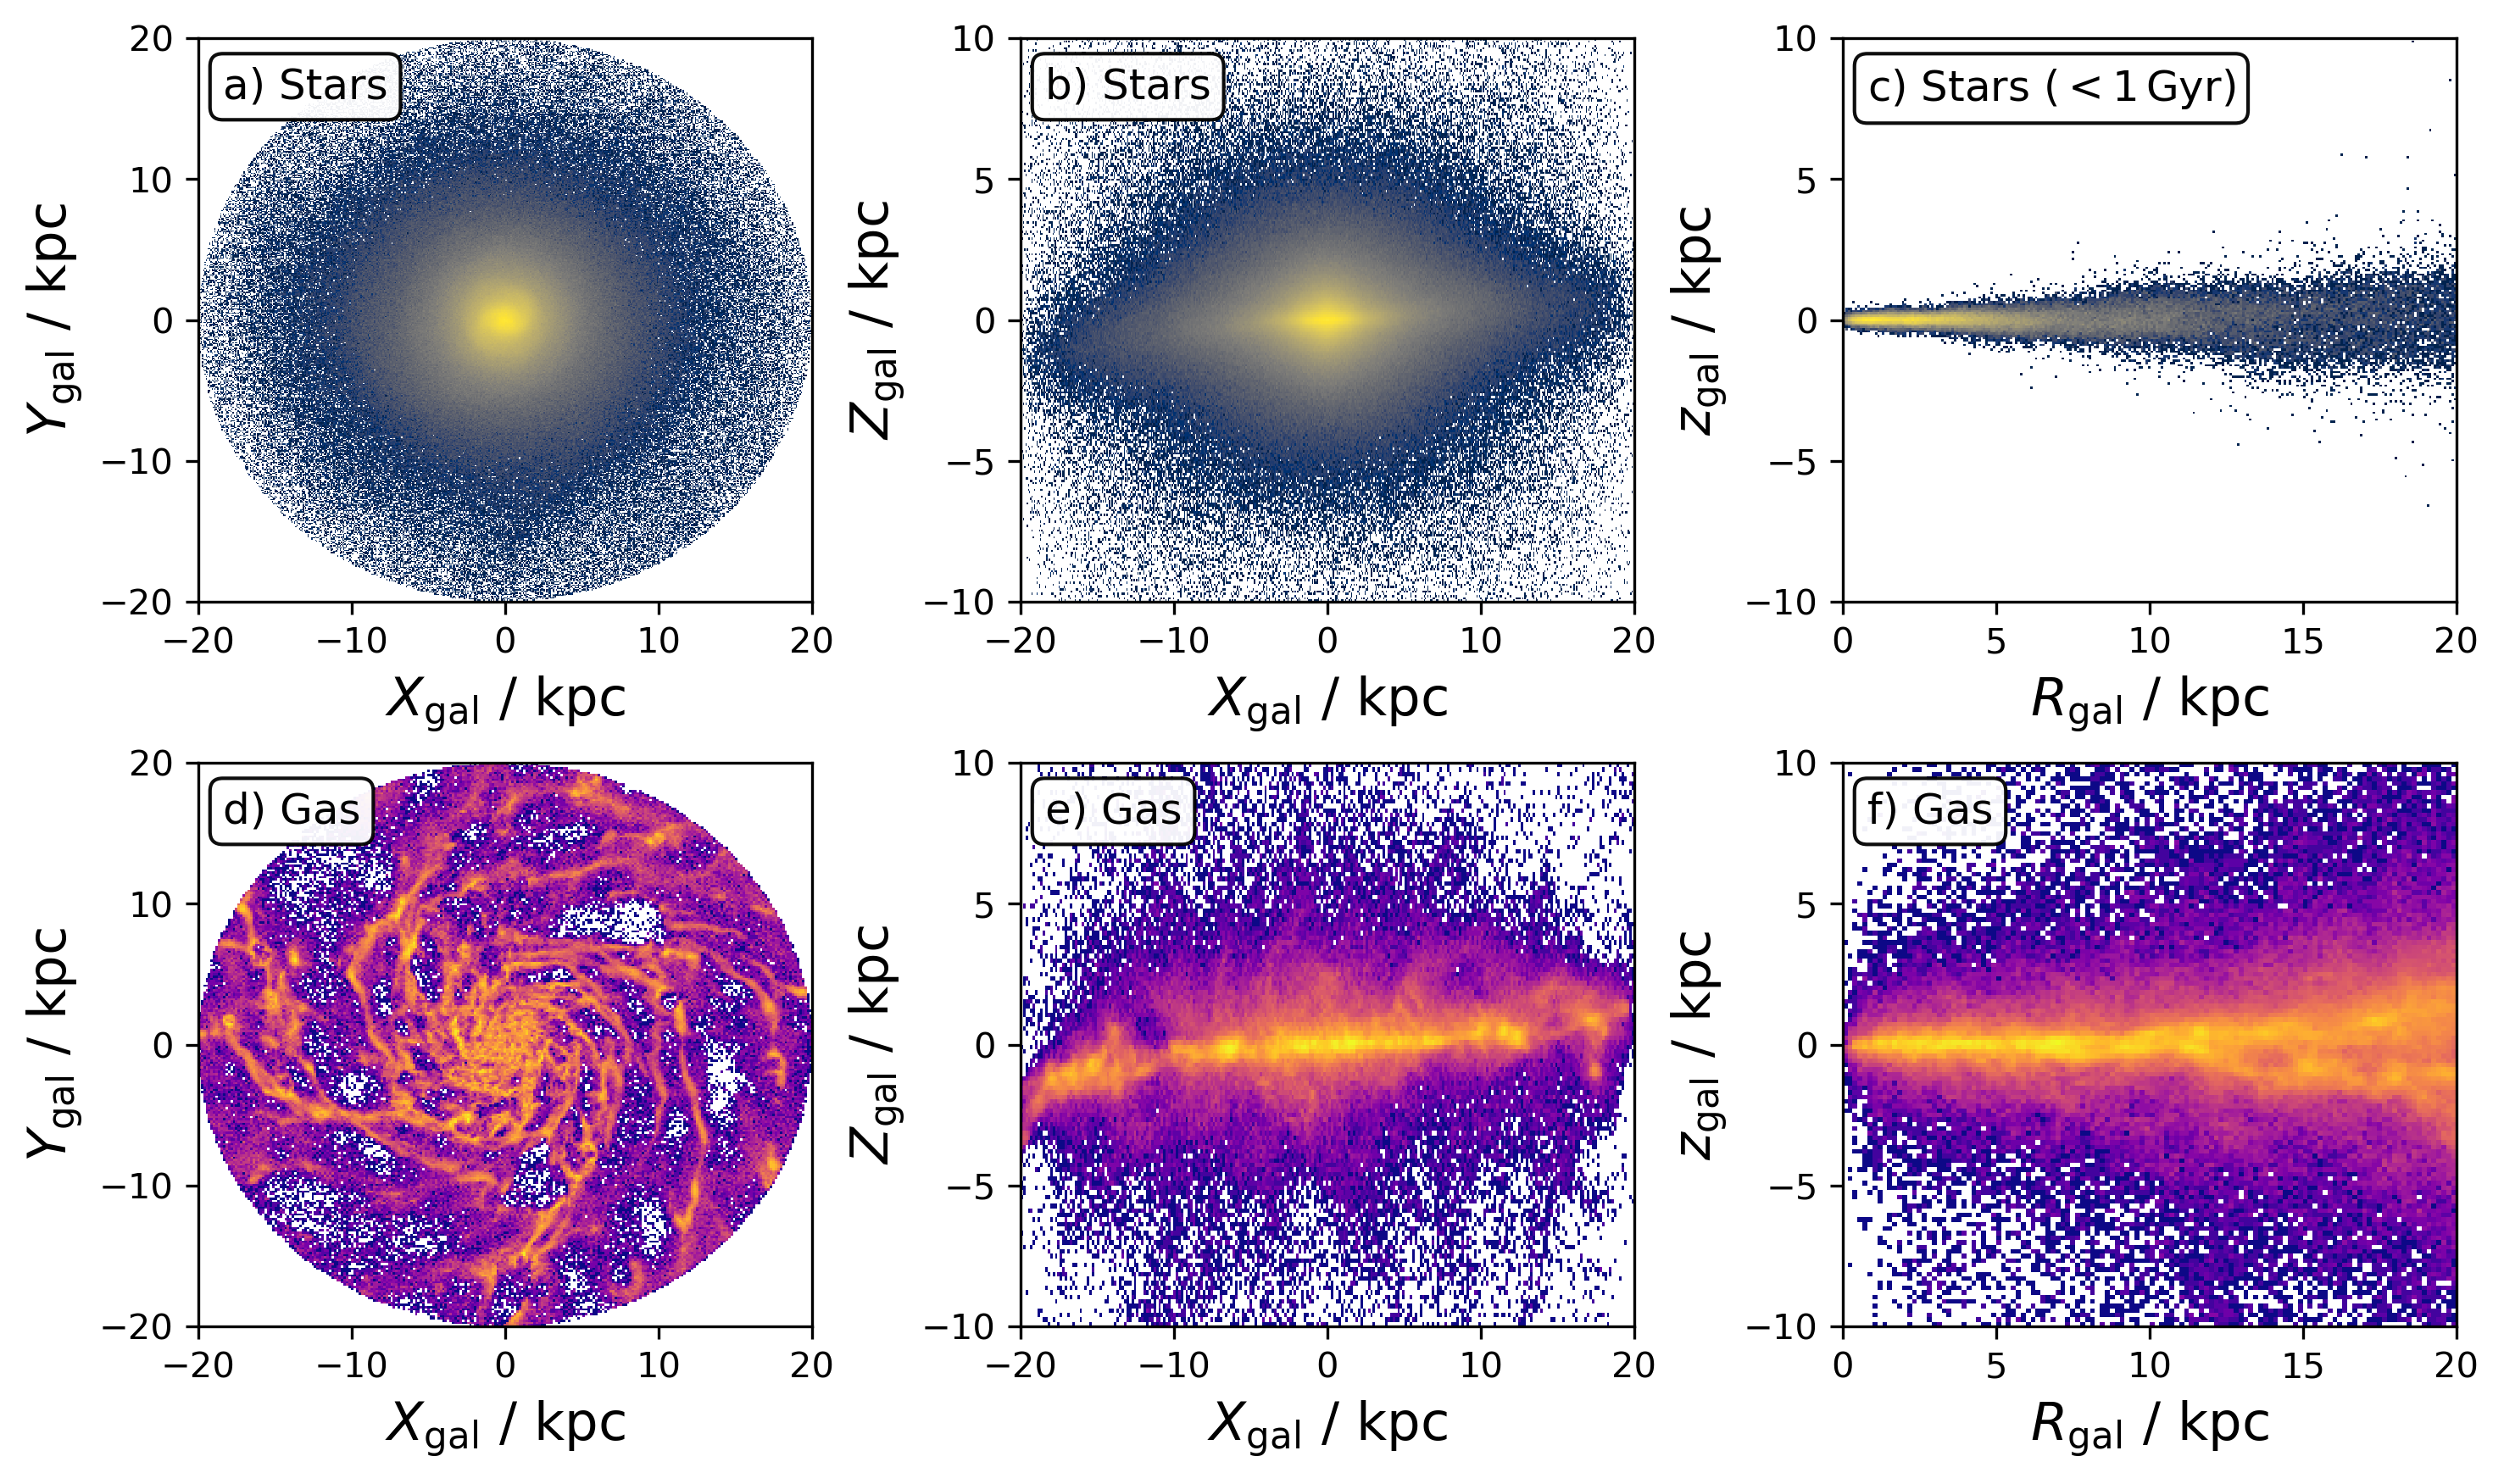
\includegraphics[width=\textwidth]{figures/stars_and_gas_overview.png}
    \caption{Logarithmic spatial density distribution of stars (upper panels) and gas (lower panels) within $R < 20\,\mathrm{kpc}$ of the NIHAO Milky Way analogue \texttt{g8.26e11} in galactocentric cartesian and cylindric coordinates. Panel c) shows the influence of selecting only young stars with ages below $1\,\mathrm{Gyr}$.}
    \label{fig:stars_and_gas_overview}
\end{figure*}

To achieve a roughly similar selection as the observational data of the Milky Way \citep{Genovali2014} and other galaxies \citep[e.g.][]{Chen2023}, we restrict the simulation data to a galactocentric radius of $R_\mathrm{Gal} \leq 20\,\mathrm{kpc}$, as shown in Fig.~\ref{fig:stars_and_gas_overview}. Similar to the Milky Way \citep{Poggio2018, Lemasle2022}, we note a warp of the stellar and gaseous disk (see Figs.~\ref{fig:stars_and_gas_overview}b and \ref{fig:stars_and_gas_overview}e, respectively).

To avoid too strong effects of radial migration \citep{Binney2008, Frankel2018} we further enforce stars to be younger than $1\,\mathrm{Gyr}$. This selection de-facto limits the vertical range of 99\% of stars to $\vert z \vert = 1.4\,\mathrm{kpc}$%. The strong influence of this age cut on the vertical distribution of stars in the Milky Way analogue can best be appreciated from the difference of vertical density distributions of stars in Figs.~\ref{fig:stars_and_gas_overview}b and \ref{fig:stars_and_gas_overview}c. We are applying these cuts for all following analyses of the radial metallicity gradient in Section~\ref{sec:radial_metallicity_gradients}.

%%%%%%%%%%%%%%%%%%%%%%%%%%%%%%%%%%%%%%%%%%%%%%%%%%

\section{The radial metallicity gradient in NIHAO}
\label{sec:radial_metallicity_gradients}

In our analysis, we follow the structure laid out with the scientific questions in Section~\ref{sec:intro}. In Section~\ref{sec:linear_radial_metallicity_gradients} we assess the linearity of the radial metallicity gradient on a global scale. In Section~\ref{sec:scatter_radial_metallicity_gradients} we quantify the scatter of the gradient. In Secs.~\ref{sec:coherence_position_radial_metallicity_gradients} and \ref{sec:coherence_age_radial_metallicity_gradients} we analyse the coherence of the gradient with position and stellar age, respectively.

\subsection{Linearity of the gradient}
\label{sec:linear_radial_metallicity_gradients}

We show the logarithmic densitry distribution of star particle iron abundances [Fe/H] across different galactocentric radii $R_\mathrm{Gal.}$ in Fig.~\ref{fig:global_r_feh_fit}a. This distribution strongly suggests that gradient is predominantly linear, similar to findings of the Milky Way.

The completeness and amount of data points on a global scale allows us, however, to probe this linearity (or more complex behaviour) in more details.

\subsubsection{Global gradient fits}


\begin{table}
\caption{Global linear gradient fit results with different methods. \textsc{LinearRegression} is part of the \textsc{sklearn} package.}
\label{tab:global_fit_results_per_method}
\begin{tabularx}{\columnwidth}{lCC}
\hline
Method & Intercept ($a_0 \pm \sigma_{a_0}$) & Slope ($a_1 \pm \sigma_{a_1}$) \\
\hline
\textsc{statsmodels.api.ODR} & $0.46229 \pm 0.00033$ & $-0.04114 \pm 0.00004$ \\
\textsc{scipy.odr} & $0.46232 \pm 0.00033$ & $-0.04114 \pm 0.00004$ \\
\textsc{np.polyfit} & $0.46229 \pm 0.00033$ & $-0.04114 \pm 0.00004$ \\
\textsc{LinearRegression} & $0.46226 \pm 0.00023$ & $-0.04112 \pm 0.00006$ \\
\hline
\end{tabularx}
\end{table}


Based on our visual inspection of Fig.~\ref{fig:global_r_feh_fit}a, we first fit a global linear radial metallicity gradient to the data. We report the gradient when using using the \textsc{LinearRegression} module of \textsc{sklearn.linear\_model} \citep{scikit-learn} in Fig.~\ref{fig:global_r_feh_fit}a as red dashed line, but have confirmed this result within the fitting uncertainties with other fitting methods (see Table~\ref{tab:global_fit_results_per_method}).

\begin{figure}
    \centering
    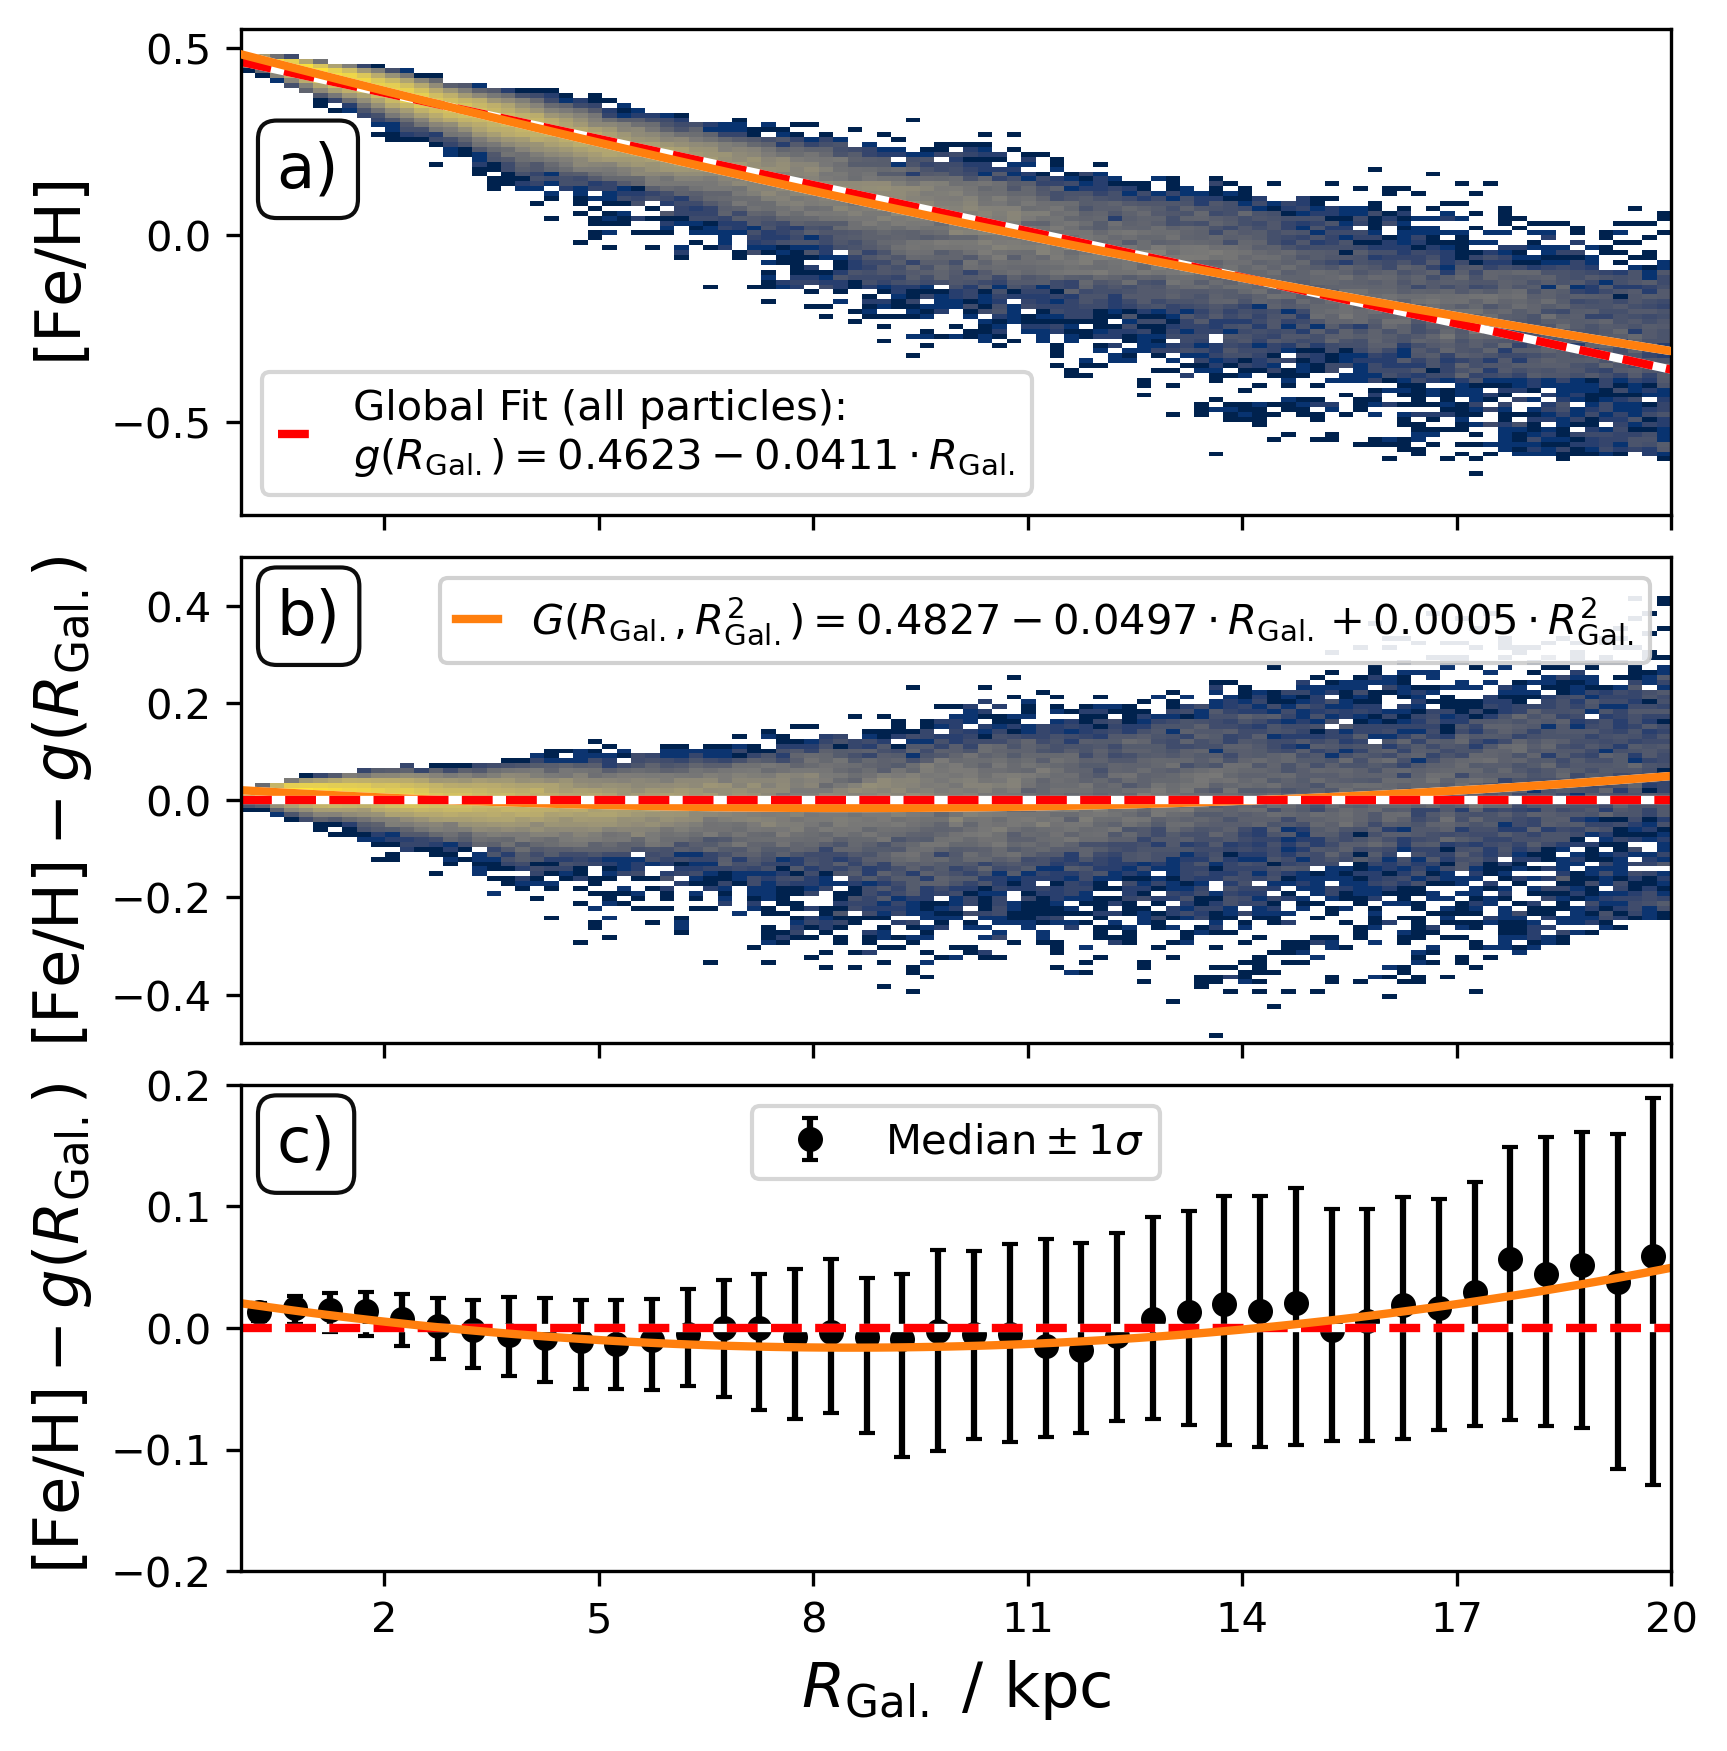
\includegraphics[width=\columnwidth]{figures/global_r_feh_fit.png}
    \caption{Global fits and deviation to the radial metallicity gradient $R-\mathrm{[Fe/H]}$. Functional forms of the linear (red) and quadratic (orange) lines are shown in the legend. Panel a) shows the underlying data of all data points as logarithmic density and the global fit to them as red dashed line. Panel b) shows the deviation of data from a linear gradient as logarithmic density plot, whereas panel c) shows the 16th and 84th percentile around the median deviation as error bars in $\Delta R_\mathrm{Gal} = 0.5\,\mathrm{kpc}$ bins.}
    \label{fig:global_r_feh_fit}
\end{figure}

We show the fit residuals in Fig.~\ref{fig:global_r_feh_fit}b as density distribution as well as in Fig.~\ref{fig:global_r_feh_fit}c as percentile distributions in radial bins of $\Delta R_\mathrm{Gal} = 0.5\,\mathrm{kpc}$. While the density distribution shows a lot of substructure, that we will investigate later, we note increase of the median residuals in Fig.~\ref{fig:global_r_feh_fit}c towards inner and outer radii, especially for $R_\mathrm{Gal.} > 17\,\mathrm{kpc}$, suggesting a non-linear component to the gradient, which we will follow up in Section~\ref{sec:non-linear_component}.

\subsubsection{The impact of radial coverage on linear fits}

While we have gained a useful insight into the global function, observational data will rarely cover the full extend of the stellar disk. Using smaller ranges, observational studies have found hints of piece-wise linear gradients with a break radius in them based on a limited radial coverage \citep[e.g.][]{Donor2020, Chen2023}.

These results are intriguing, since a quadratic function can to first order be approximated by two linear functions with a break radius. We therefore want to use this simulation to test if the radial coverage may indeed delude us into identifying broken linear gradients.

\begin{figure}
    \centering
    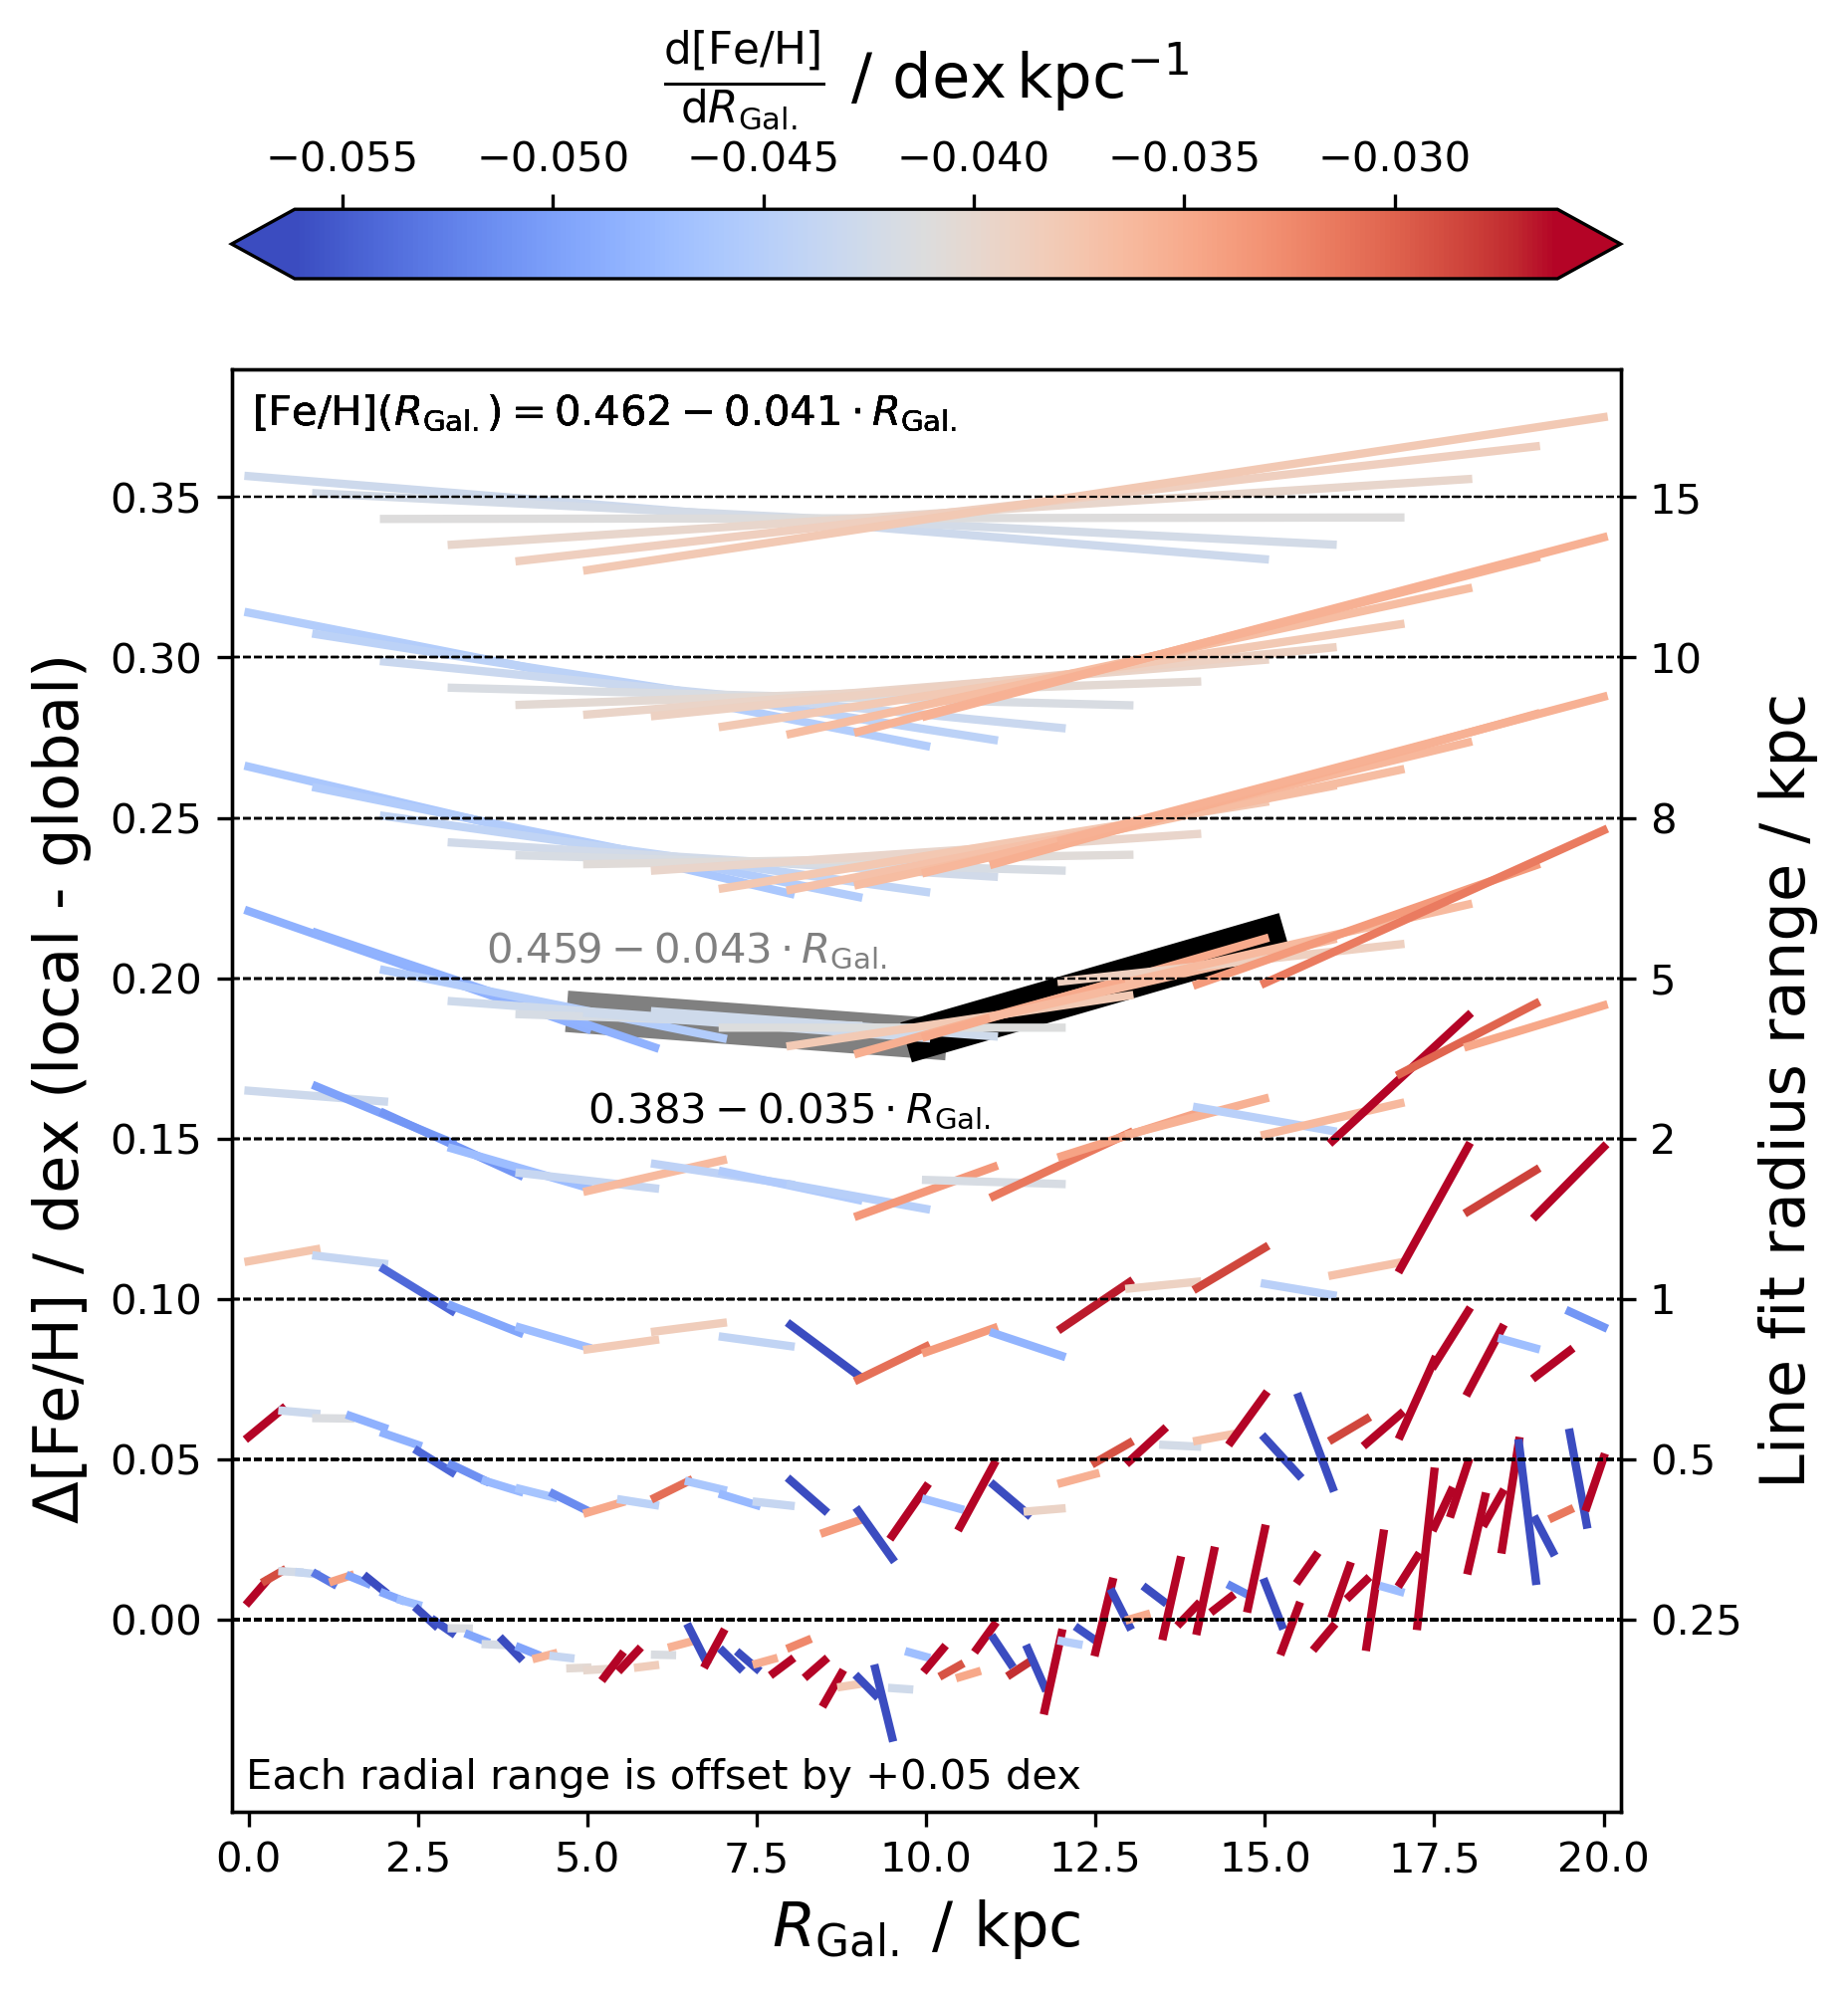
\includegraphics[width=\columnwidth]{figures/radial_range_impact.png}
    \caption{Impact of different coverage in galactocentric radius when fitting a linear radial metallicity gradient to young stars. Each horizontal segment is using a different running radial fitting range between 0.25 and $15\,\mathrm{kpc}$ as outlined on the right. For better contrast, the global linear fit is subtracted from the local gradient estimates and each line is colored by the gradient slope with a color scale centered around the global fit slope.}
    \label{fig:radial_range_impact}
\end{figure}

For this purpose, we are fitting and comparing linear radial metallicity gradients to subsets in galactocentric radius. We test fits across piecewise linear radial ranges of 0.25, 0.5, 1, 2, 5, 8, 10, 15, and $20\,\mathrm{kpc}$ and show their difference with respect to a global linear fit in Fig.~\ref{fig:radial_range_impact}, with color-coding and indicating the local gradient slope. In this figure, a horizontal line indicates the same slope as the global fit, whereas the offset of a line from the horizontal dashed line indicates the local deviation from the global gradient. We see that all ranges do suggest more or less significant deviations from a global linear fit, with the innermost fit suggesting a significantly different gradient than the outermost fit. We also note increasingly more slope differences towards the smallest scales, hinting at local deviations from a global pattern. We follow these up in Section~\ref{sec:scatter_radial_metallicity_gradients}, but for now focus on the larger-scale trends.

When directly comparing an inner and outer radius fit, such as between $R_\mathrm{Gal.} = 5-10\,\mathrm{kpc}$ (thick grey line in Fig.~\ref{fig:radial_range_impact}) and $R_\mathrm{Gal.} = 10-15\,\mathrm{kpc}$ (thick black line in Fig.~\ref{fig:radial_range_impact}), we note a significant change, similar to previous estimates of the Milky Way \citep[e.g.][]{Lemasle2008}. In our case the gradient estimate changes from $\mathrm{[Fe/H]}(R_\mathrm{Gal.}) = 0.471-0.044\cdot R_\mathrm{Gal.}$%
 to $\frac{\mathrm{d[Fe/H]}}{\mathrm{d}R_\mathrm{Gal.}} = 0.383-0.035\cdot R_\mathrm{Gal.}$%
.

\subsubsection{Higher-order gradients} \label{sec:non-linear_component}

From the previous section, and especially the changing deviation of local gradients from a global fit in Fig.~\ref{fig:radial_range_impact}, we acknowledge that a linear fit is - not unexpected - not able to capture the more intricate details of the radial abundance gradient. In particular, we realise that the abundance gradient is indeed flattening - even for stars with young ages ($< 1\,\mathrm{Gyr}$). When looking at linear gradient fits across radial coverages of  $\Delta R_\mathrm{Gal.} = 5-15\,\mathrm{kpc}$ in Fig.~\ref{fig:radial_range_impact}, the gradient was steeper (bluer color) for smaller radii and flatter (redder) for larger radii.

While such effects have seen before for the Milky Way, previous studies how mostly suggested to fit piecewise linear gradients with a break radius \citep[e.g.][]{Andrievsky2002, Boeche2013, Hayden2014, Anders2017, Donor2020}.

Our results from Fig.~\ref{fig:radial_range_impact} suggest, however, not one break radius, but rather an smoothly evolving flattening, in better agreement with a quadratic function rather than two linear ones. In this section, we are therefore trying to expand the gradient function by a higher order, that is second order, one.

A quadratic fit (see orange lines in Fig.~\ref{fig:global_r_feh_fit}) results in a slightly steeper linear component of the gradient (from $-0.0411$ to $-0.0497\,\mathrm{dex\,kpc^{-1}}$), which is counteracted by the quadratic flattening term of $+0.0005\,\mathrm{dex\,kpc^{-2}}$. The latter leads to an effective flattening of $0.2\,\mathrm{dex}$ at $R_\mathrm{Gal.} = 20\,\mathrm{dex}$. While seemingly only a nuisance correction across the large extend of [Fe/H] and $R_\mathrm{Gal.}$, this quadratic function is in fact superior to the linear fit. This can be best appreciated in Fig.~\ref{fig:global_r_feh_fit}c, where the orange line is tracing the median residuals from the linear function much better across the all radii.

\begin{figure}
    \centering
    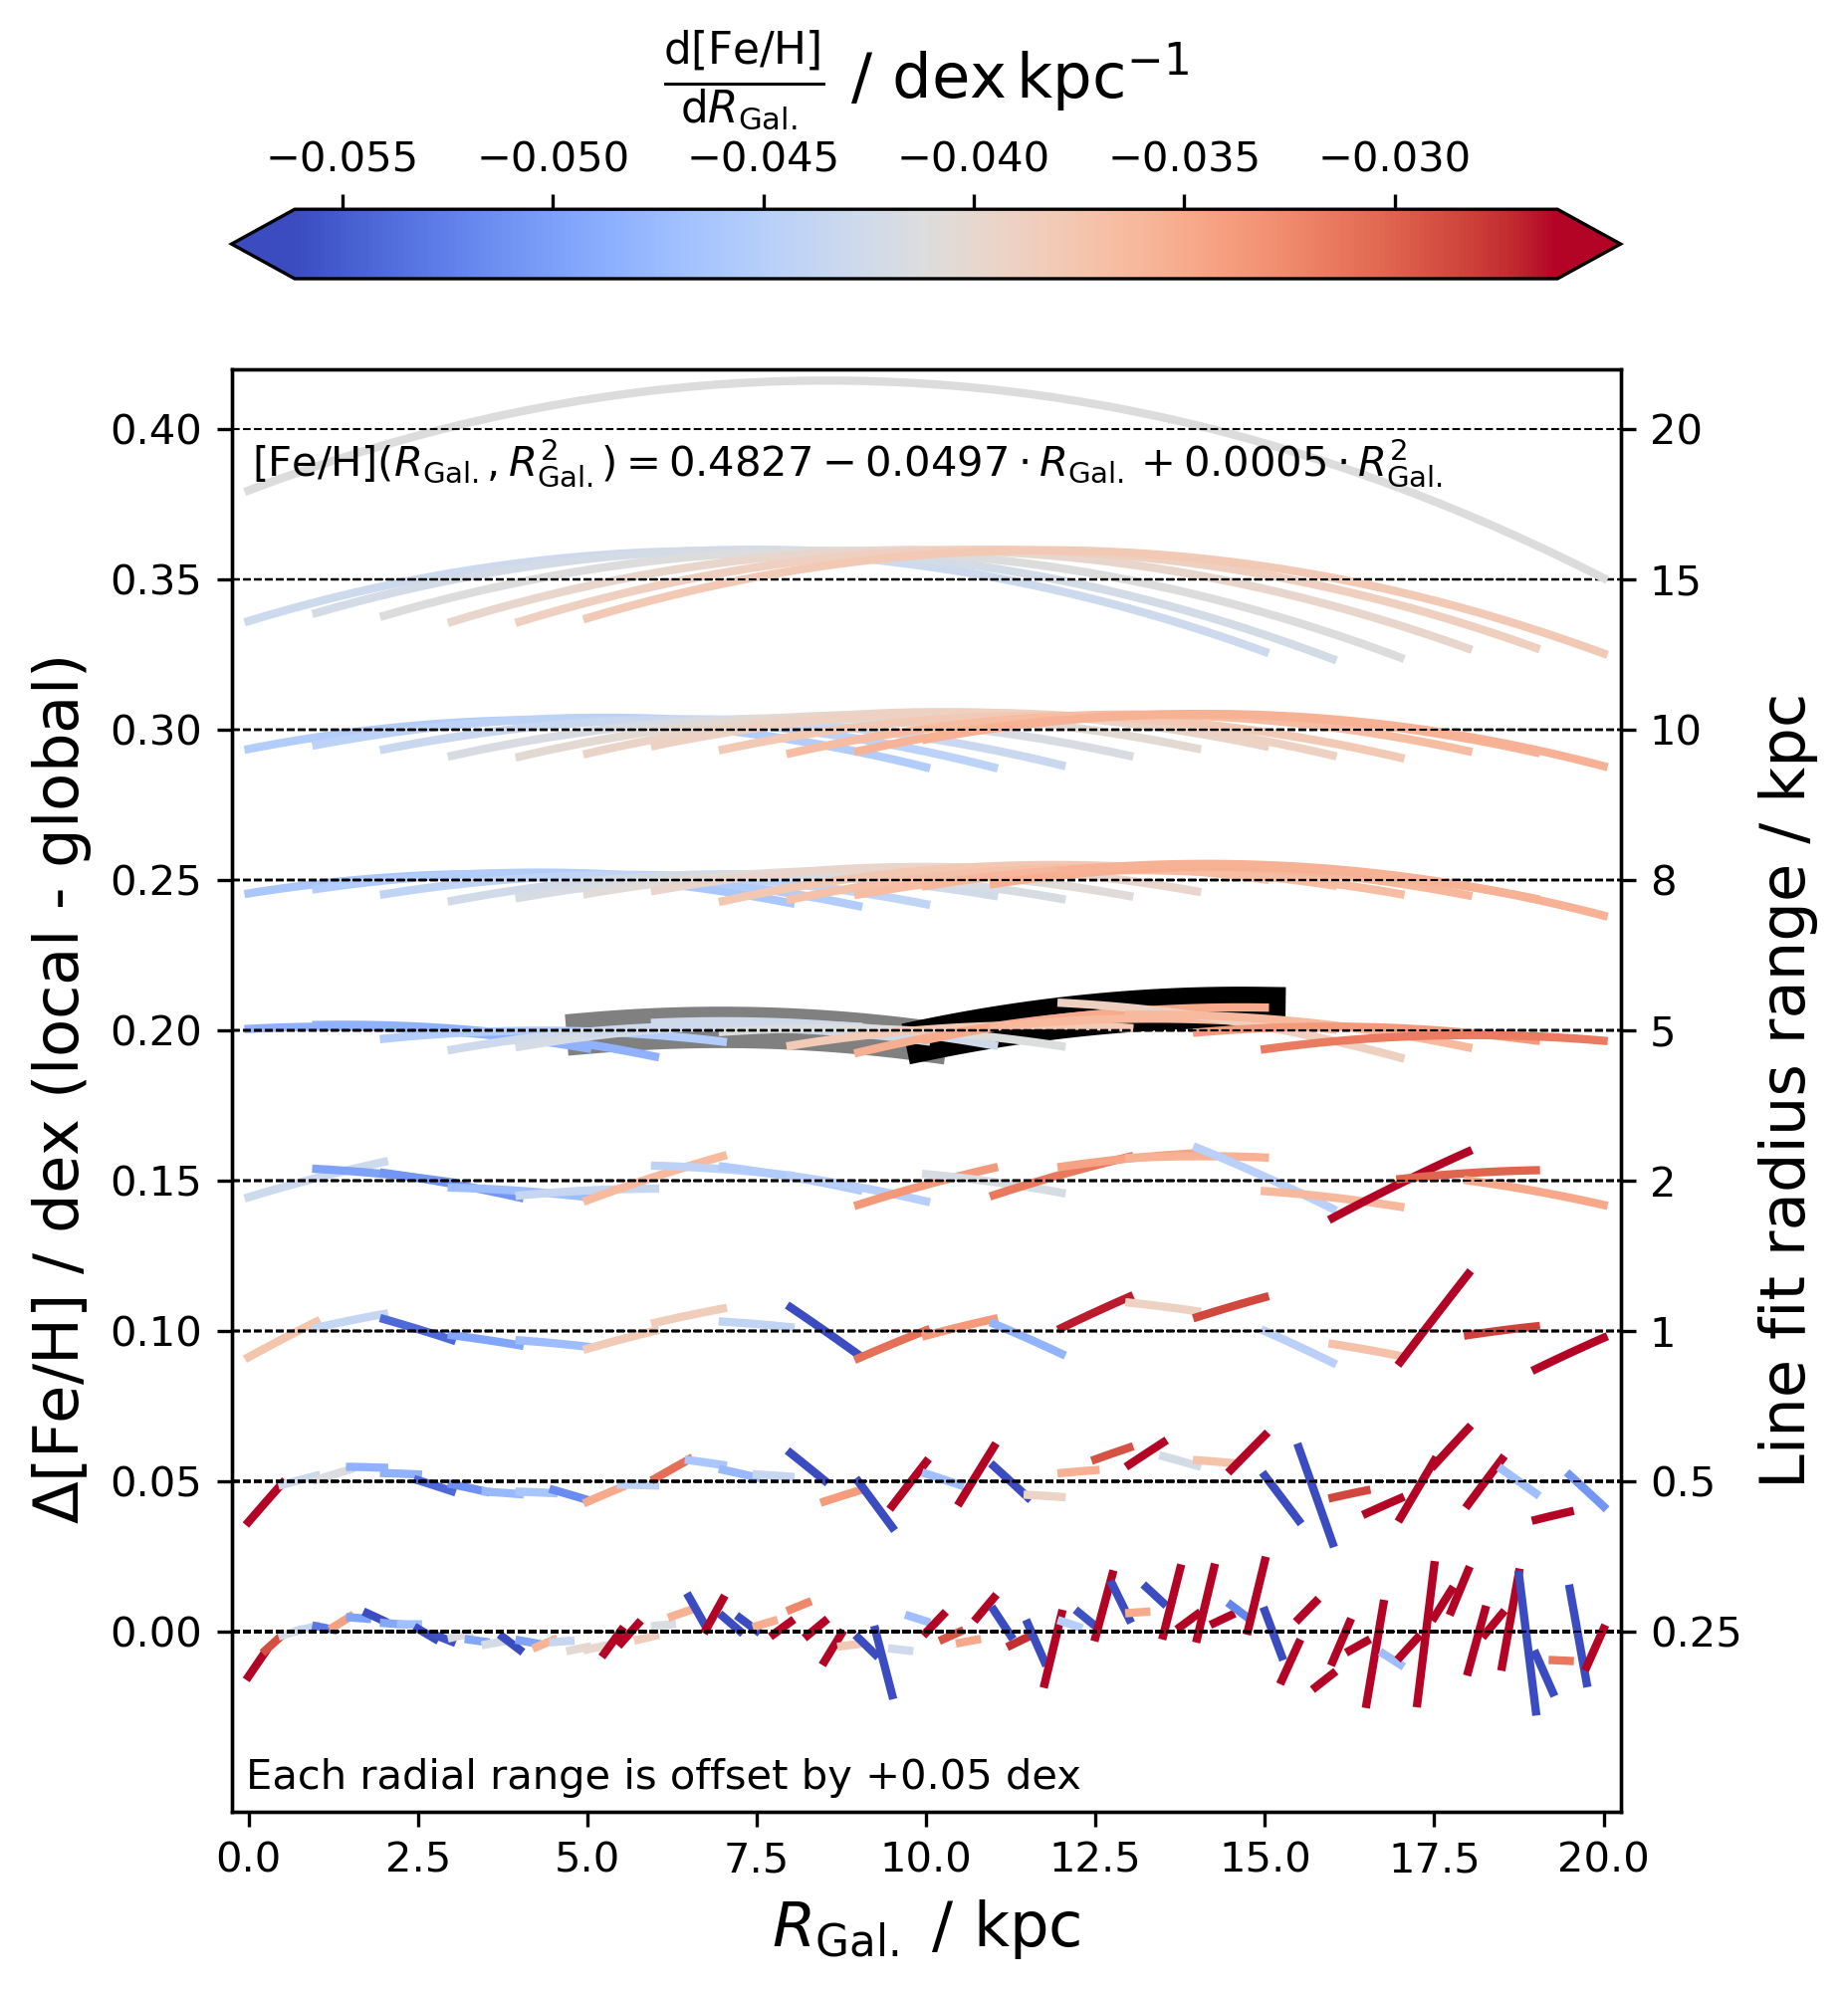
\includegraphics[width=\columnwidth]{figures/radial_range_impact_quadratic.png}
    \caption{Same as Fig.~\ref{fig:radial_range_impact}, but comparing local deviations to a quadratic global fit. Overall deviations have decreased most notably for innermost and outermost radii.}
    \label{fig:radial_range_impact_quadratic}
\end{figure}

When reproducing the local deviations from the linear global fit (Fig.~\ref{fig:radial_range_impact}) with a quadratic global fit (Fig.~\ref{fig:radial_range_impact_quadratic}), we see that the deviations of the local fits no longer have significant offsets with respect to the horizontal lines, while still showing the increasing slope differences at the local levels (especially on scales below $1\,\mathrm{kpc}$). 

\subsection{Scatter and local deviations from the gradient}
\label{sec:scatter_radial_metallicity_gradients}

Now that we are sufficiently satisfied that our flattening linear gradient reproduces the overall shape of the radial metallicity gradient, we \SB{CONTINUE}

see Fig.~\ref{fig:overlap_local_variation_gas} -> maybe something to do with gas density and or logal variations of gas? should we maybe also plot the star positions here to check for differences or $R-z$ for stars? YES!

\begin{figure}
    \centering
    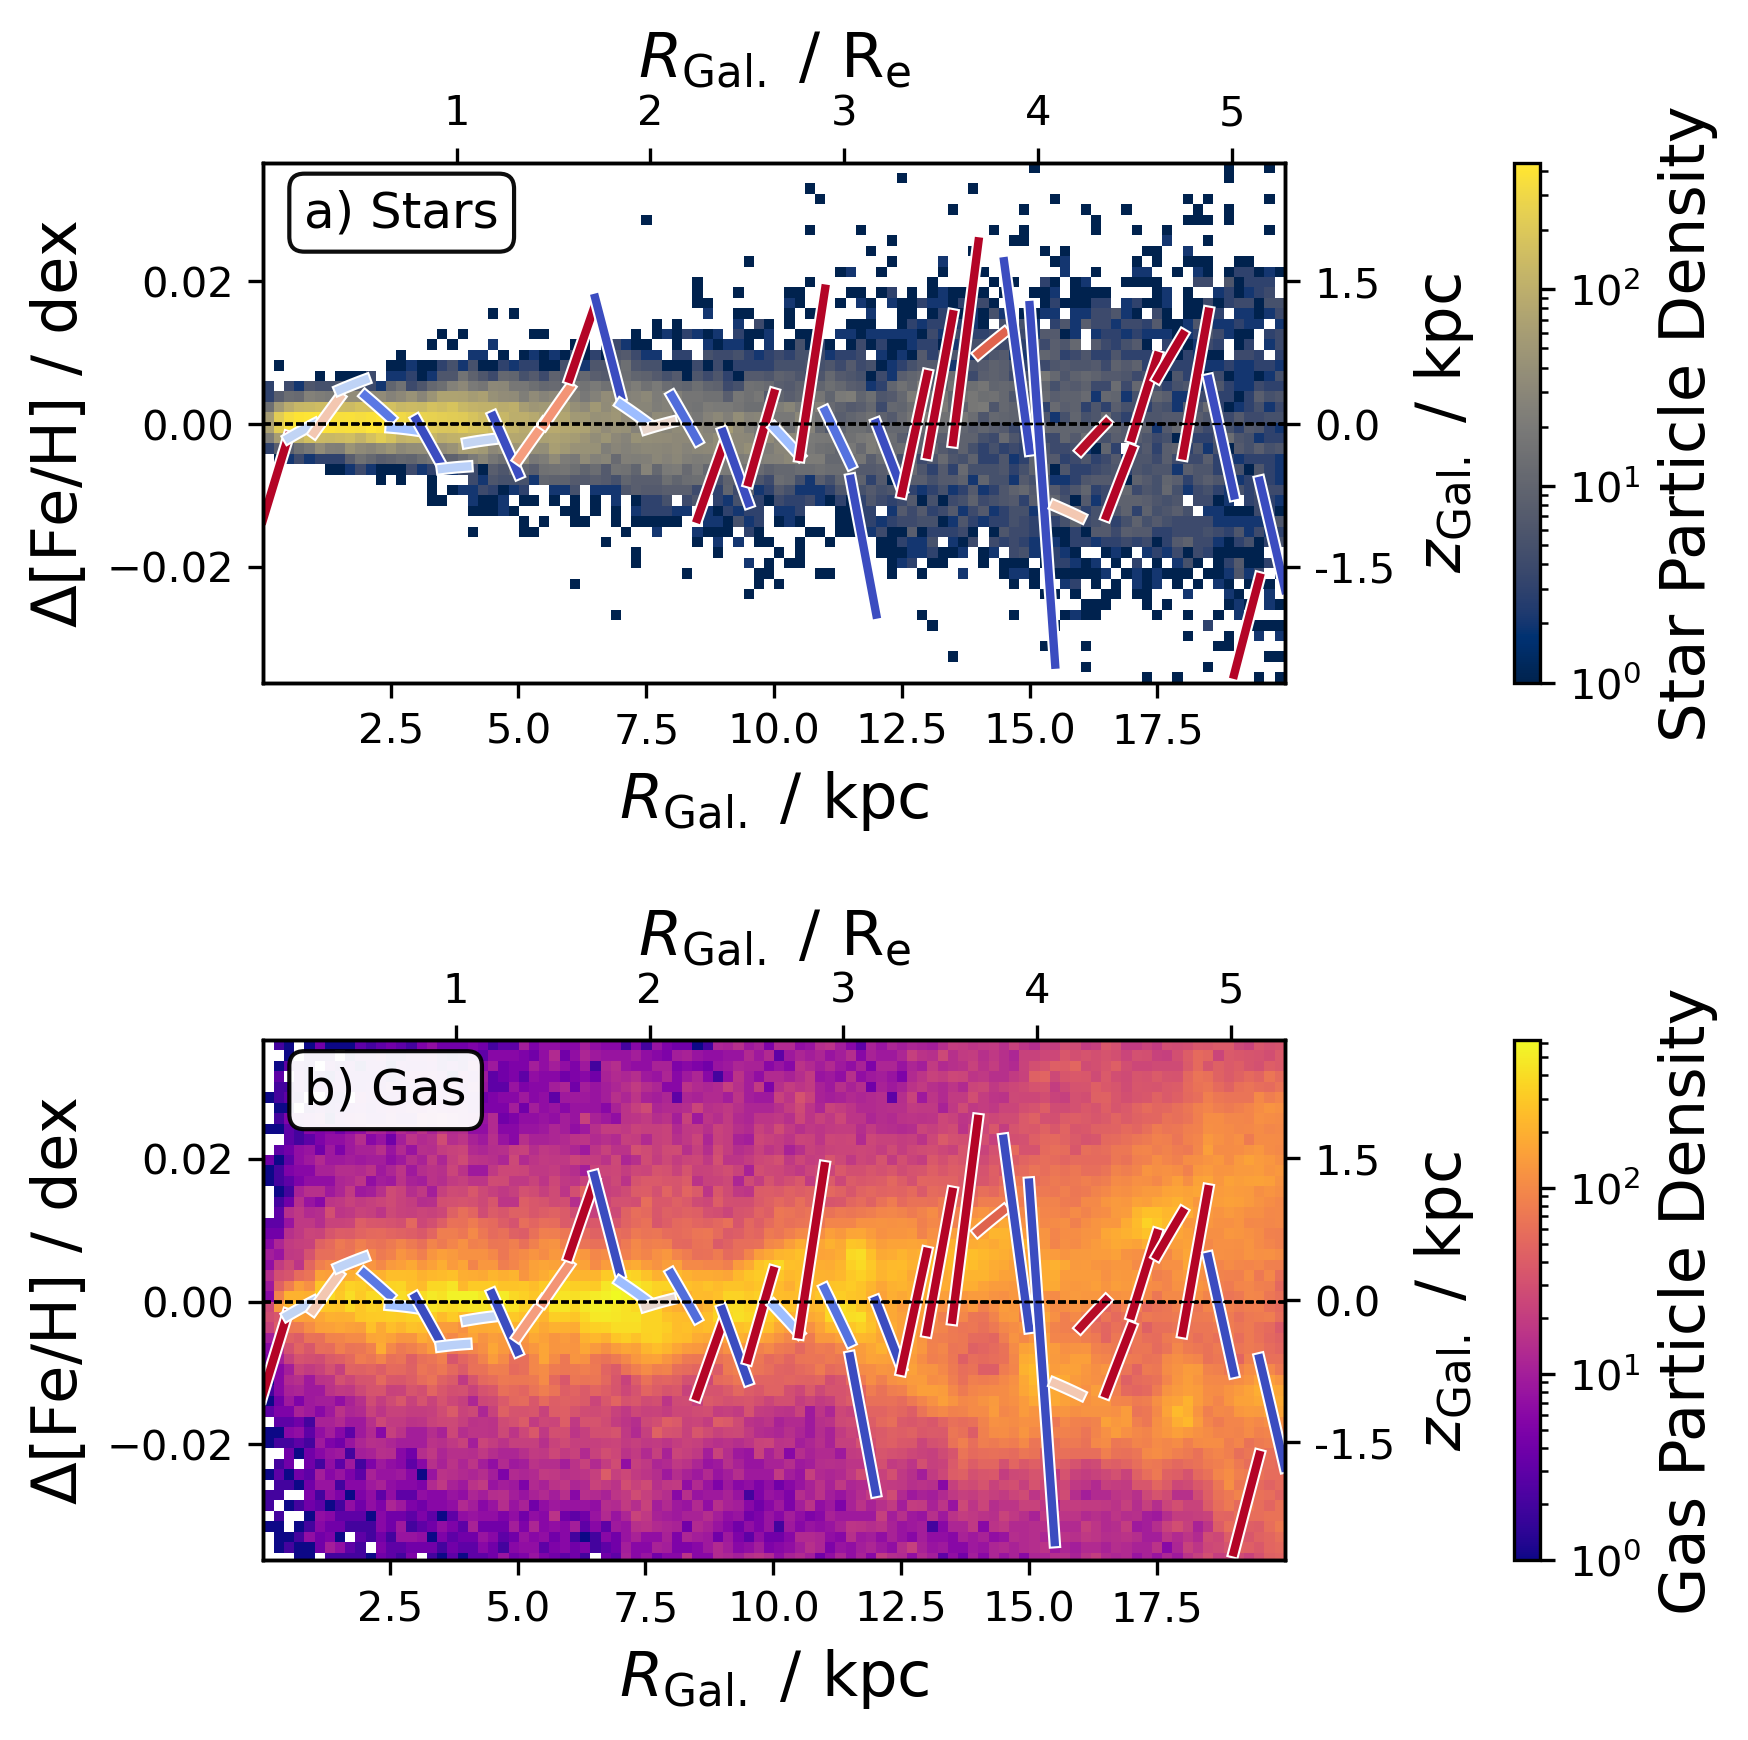
\includegraphics[width=\columnwidth]{figures/overlap_local_variation_gas.png}
    \caption{Local gradient deviations from bottom row of Fig.~\ref{fig:radial_range_impact_quadratic} overlapped on the logarithmic density distribution of gas in $R-z$.}
    \label{fig:overlap_local_variation_gas}
\end{figure}


\SB{How significant is the difference of linear to quadratic when looking at 5-19 kpc, like MW studies \citep{Genovali2014}?}


Motivated by the significant spread of open cluster metallicities at the solar radius beyond observational uncertainty \citep[e.g.][]{Donor2020, Spina2021}, we are now turning to the scatter of the radial metallicity gradient.

In this section, we investigate
\begin{itemize}
    \item the change of scatter from the innermost radii to the outermost (see Fig.~\ref{fig:global_r_feh_fit}c). We see a steady increase in $1-\sigma$ spread of $\sigma \mathrm{[Fe/H]} = 0.01\,\mathrm{dex}$%
 at $R_\mathrm{Gal.} = 0.25 \pm 0.25\,\mathrm{kpc}$, $\sigma \mathrm{[Fe/H]} = 0.06\,\mathrm{dex}$%
 at $R_\mathrm{Gal.} = 8.25 \pm 0.25\,\mathrm{kpc}$, to $\sigma \mathrm{[Fe/H]} = 0.10\,\mathrm{dex}$%
 at $R_\mathrm{Gal.} = 19.5 \pm 0.25\,\mathrm{kpc}$.
\end{itemize}

Do the young stars actually trace the gas? See Fig.~\ref{fig:tracing_young_stars_and_gas_in_angles}

\begin{figure}
    \centering
    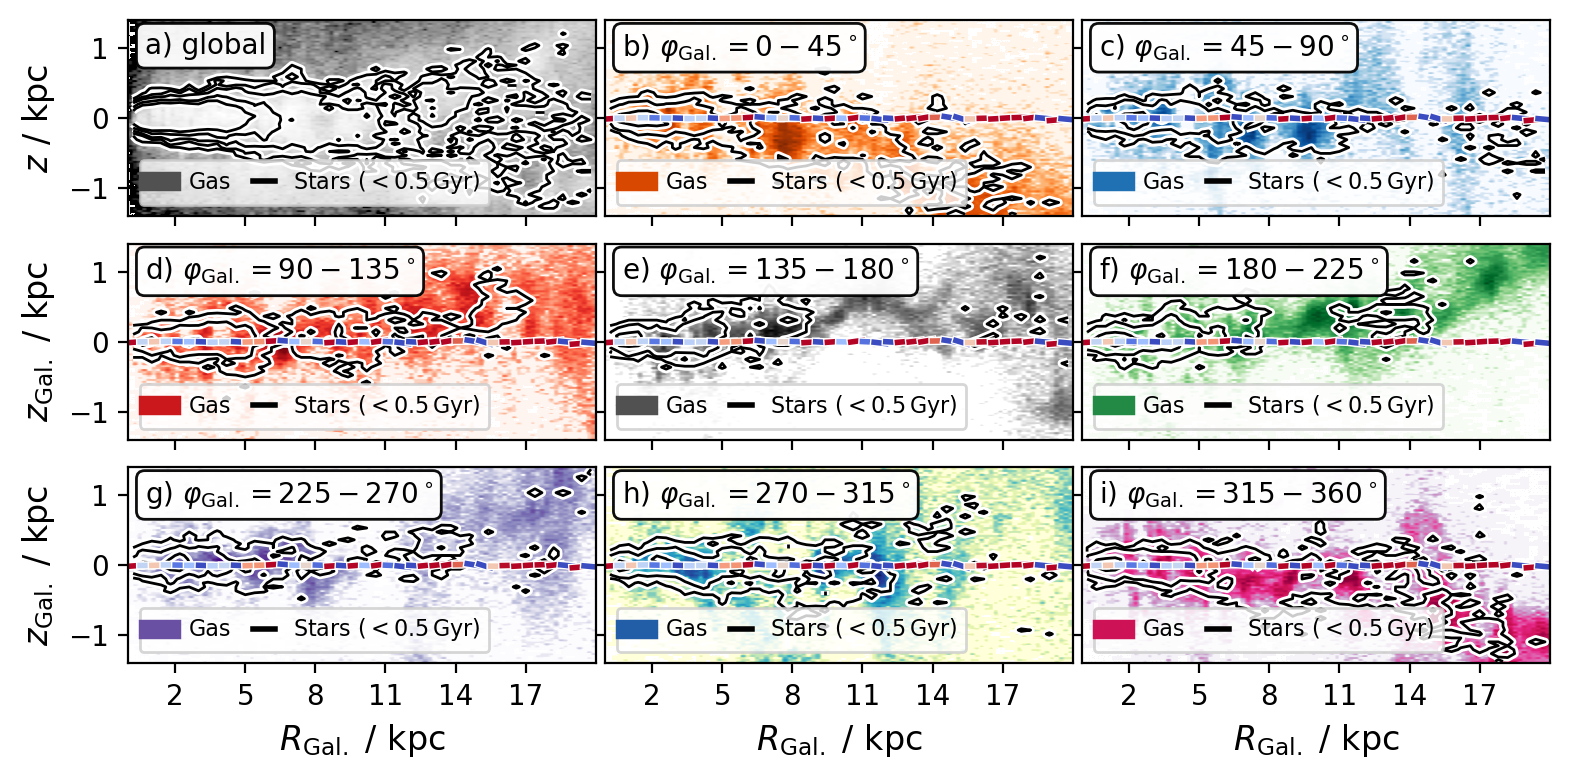
\includegraphics[width=\columnwidth]{figures/tracing_young_stars_and_gas_in_angles.png}
    \caption{Tracing young stars and gas across the galaxy (panel a) and different azimuthal ranges (panels b-i).}
    \label{fig:tracing_young_stars_and_gas_in_angles}
\end{figure}




\subsection{Coherence of the gradient with position}
\label{sec:coherence_position_radial_metallicity_gradients}

\begin{itemize}
    \item Density variation of the radial metallicity gradient $R-\mathrm{[Fe/H]}$ across 8 different sectors in Fig.~\ref{fig:radial_metallicity_gradients_mw_in_angles}
    \item Deviation from global radial metallicity gradient across 8 different sectors in Fig.~\ref{fig:linear_radial_metallicity_gradients_mw_in_angles}
    \item Compute gradient over a radius R and then plot this one in color in the xy direction (like hogg/eilers). Maybe 2kpc is the best radius to do that? Can also try 5kpc.
\end{itemize}

\begin{figure*}
    \centering
    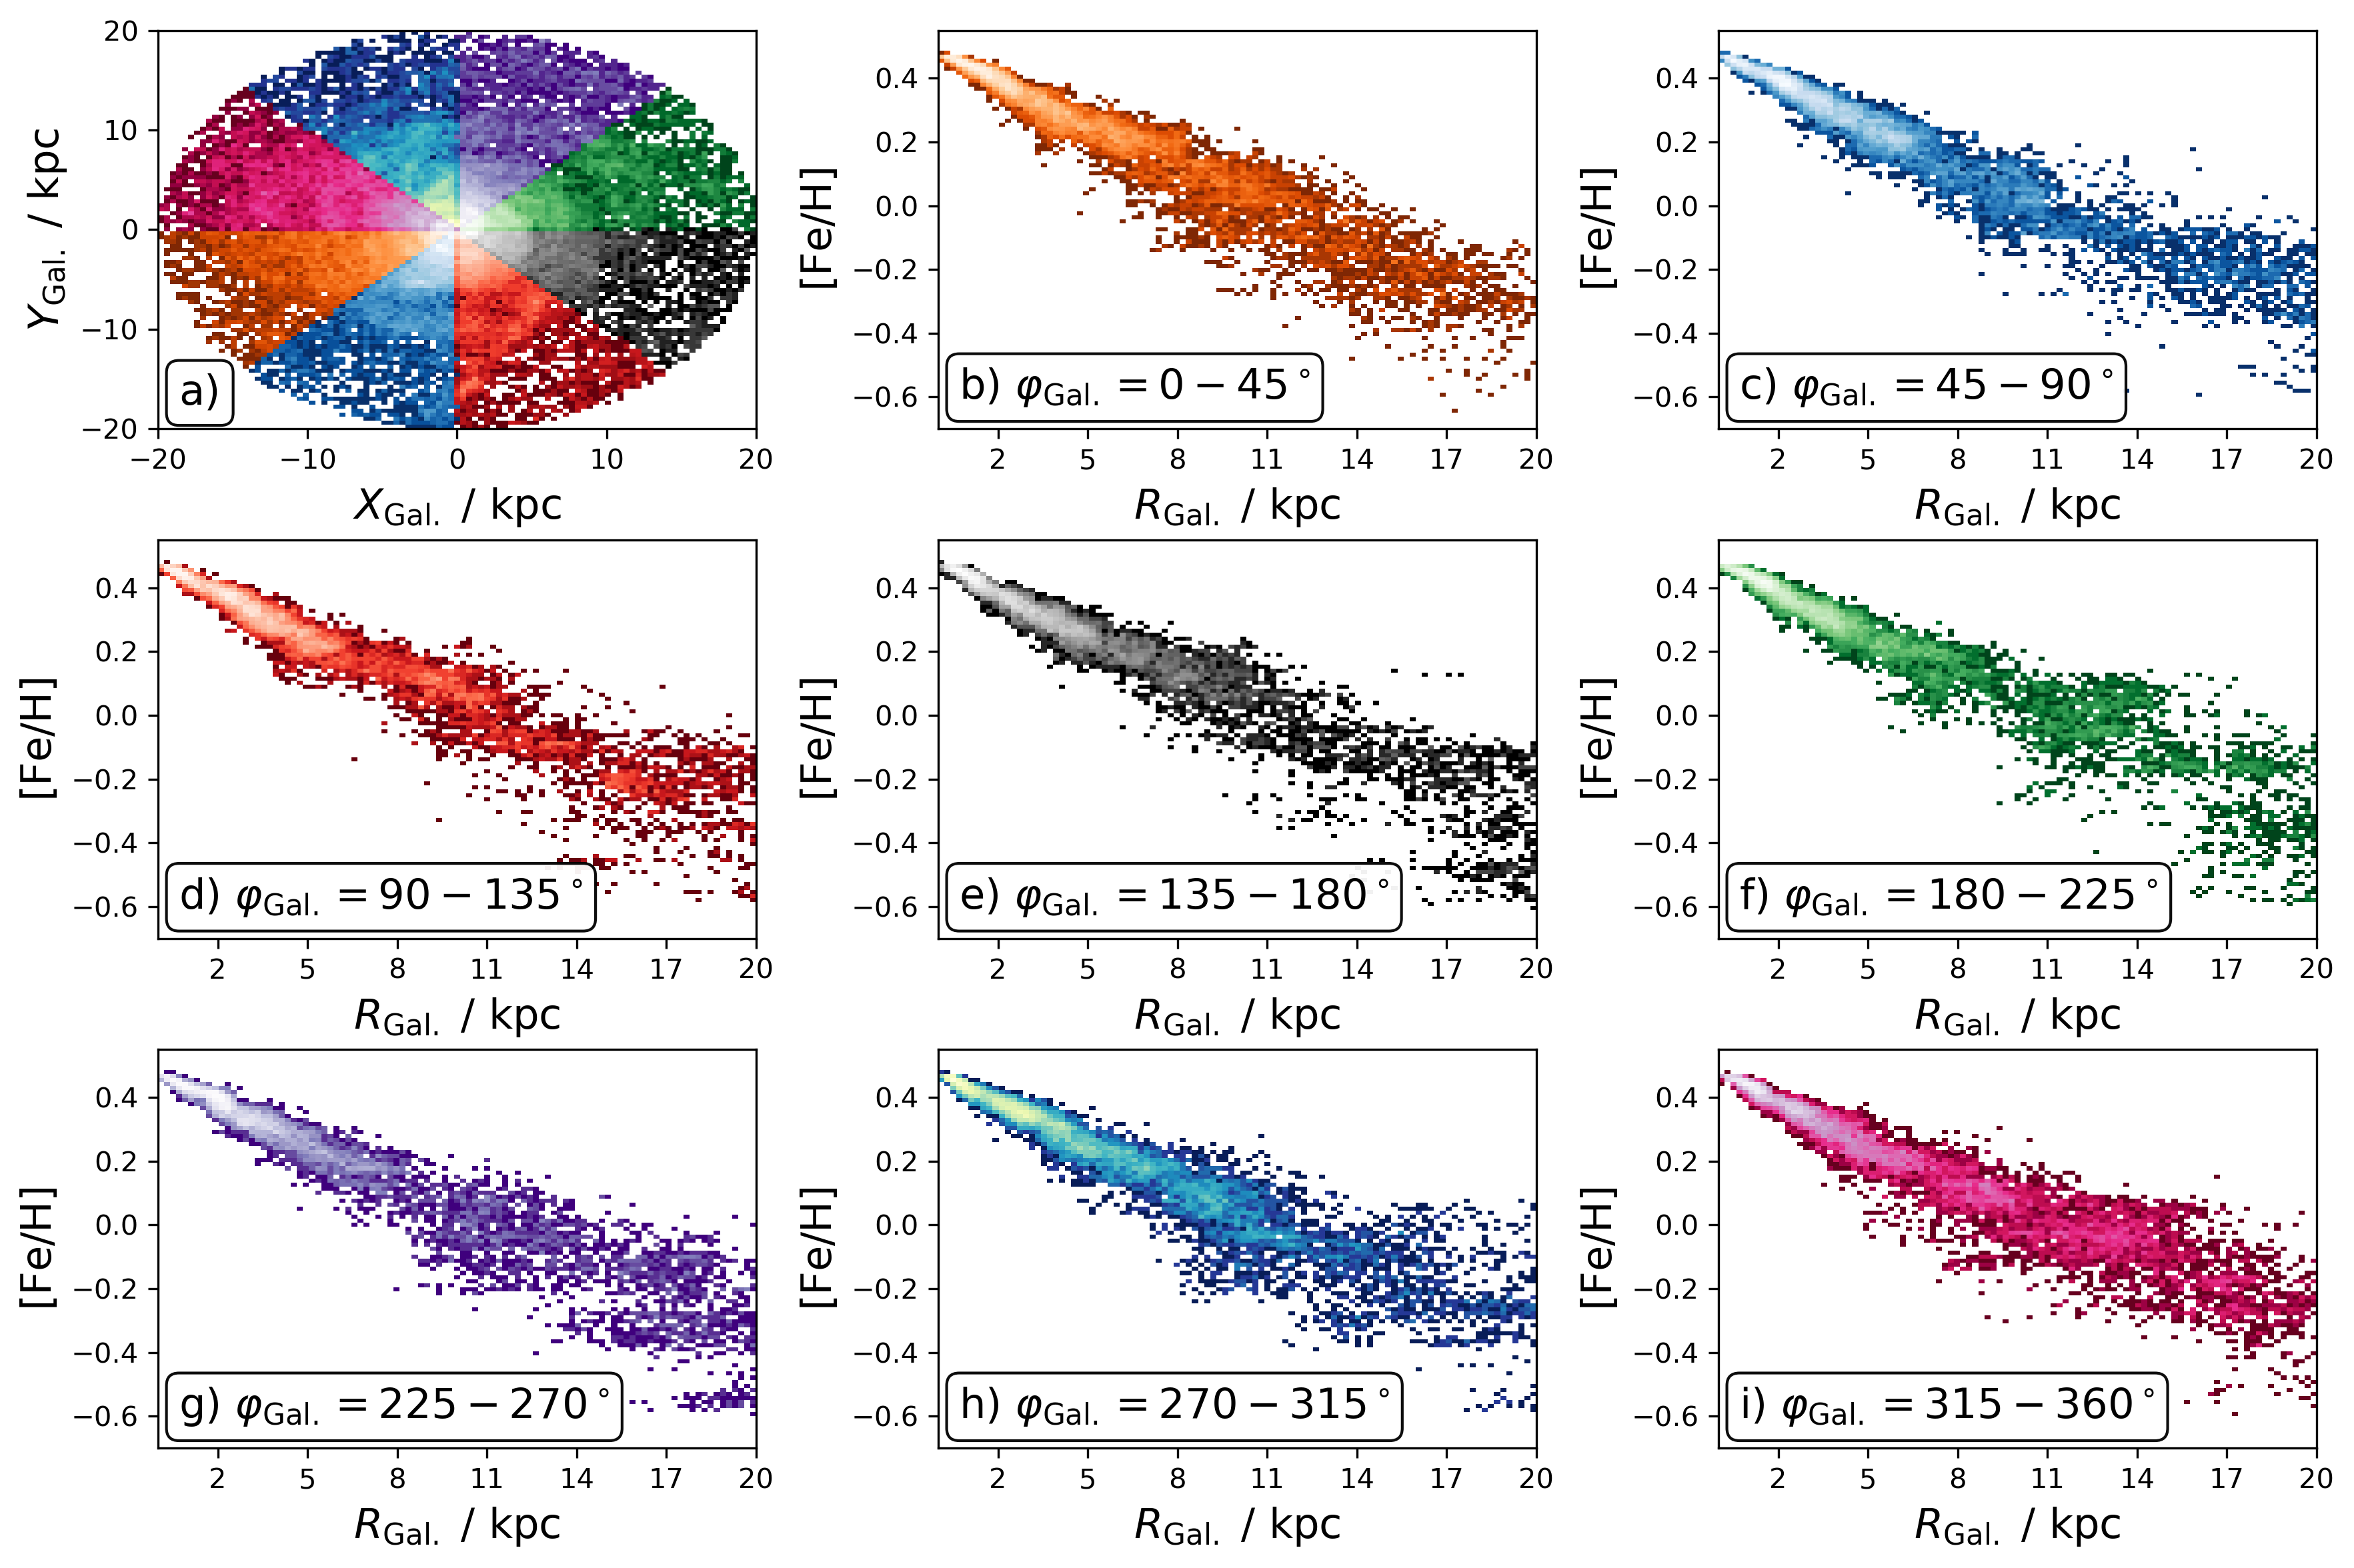
\includegraphics[width=\textwidth]{figures/radial_metallicity_gradients_mw_in_angles.png}
    \caption{Density variation across 8 different sectors (with color-code visualised in panel a) of the radial metallicity gradient $R-\mathrm{[Fe/H]}$ across 8 different azimuth ranges (panels b-i). A rotating lighthouse-like GIF animation of the median age and median density of the $R-\mathrm{[Fe/H]}$-relation is freely available on the \href{https://github.com/svenbuder/nihao_radial_metallicity_gradients/blob/main/figures/xyz_rfeh.gif}{github repository}.}
    \label{fig:radial_metallicity_gradients_mw_in_angles}
\end{figure*}

\begin{figure*}
    \centering
    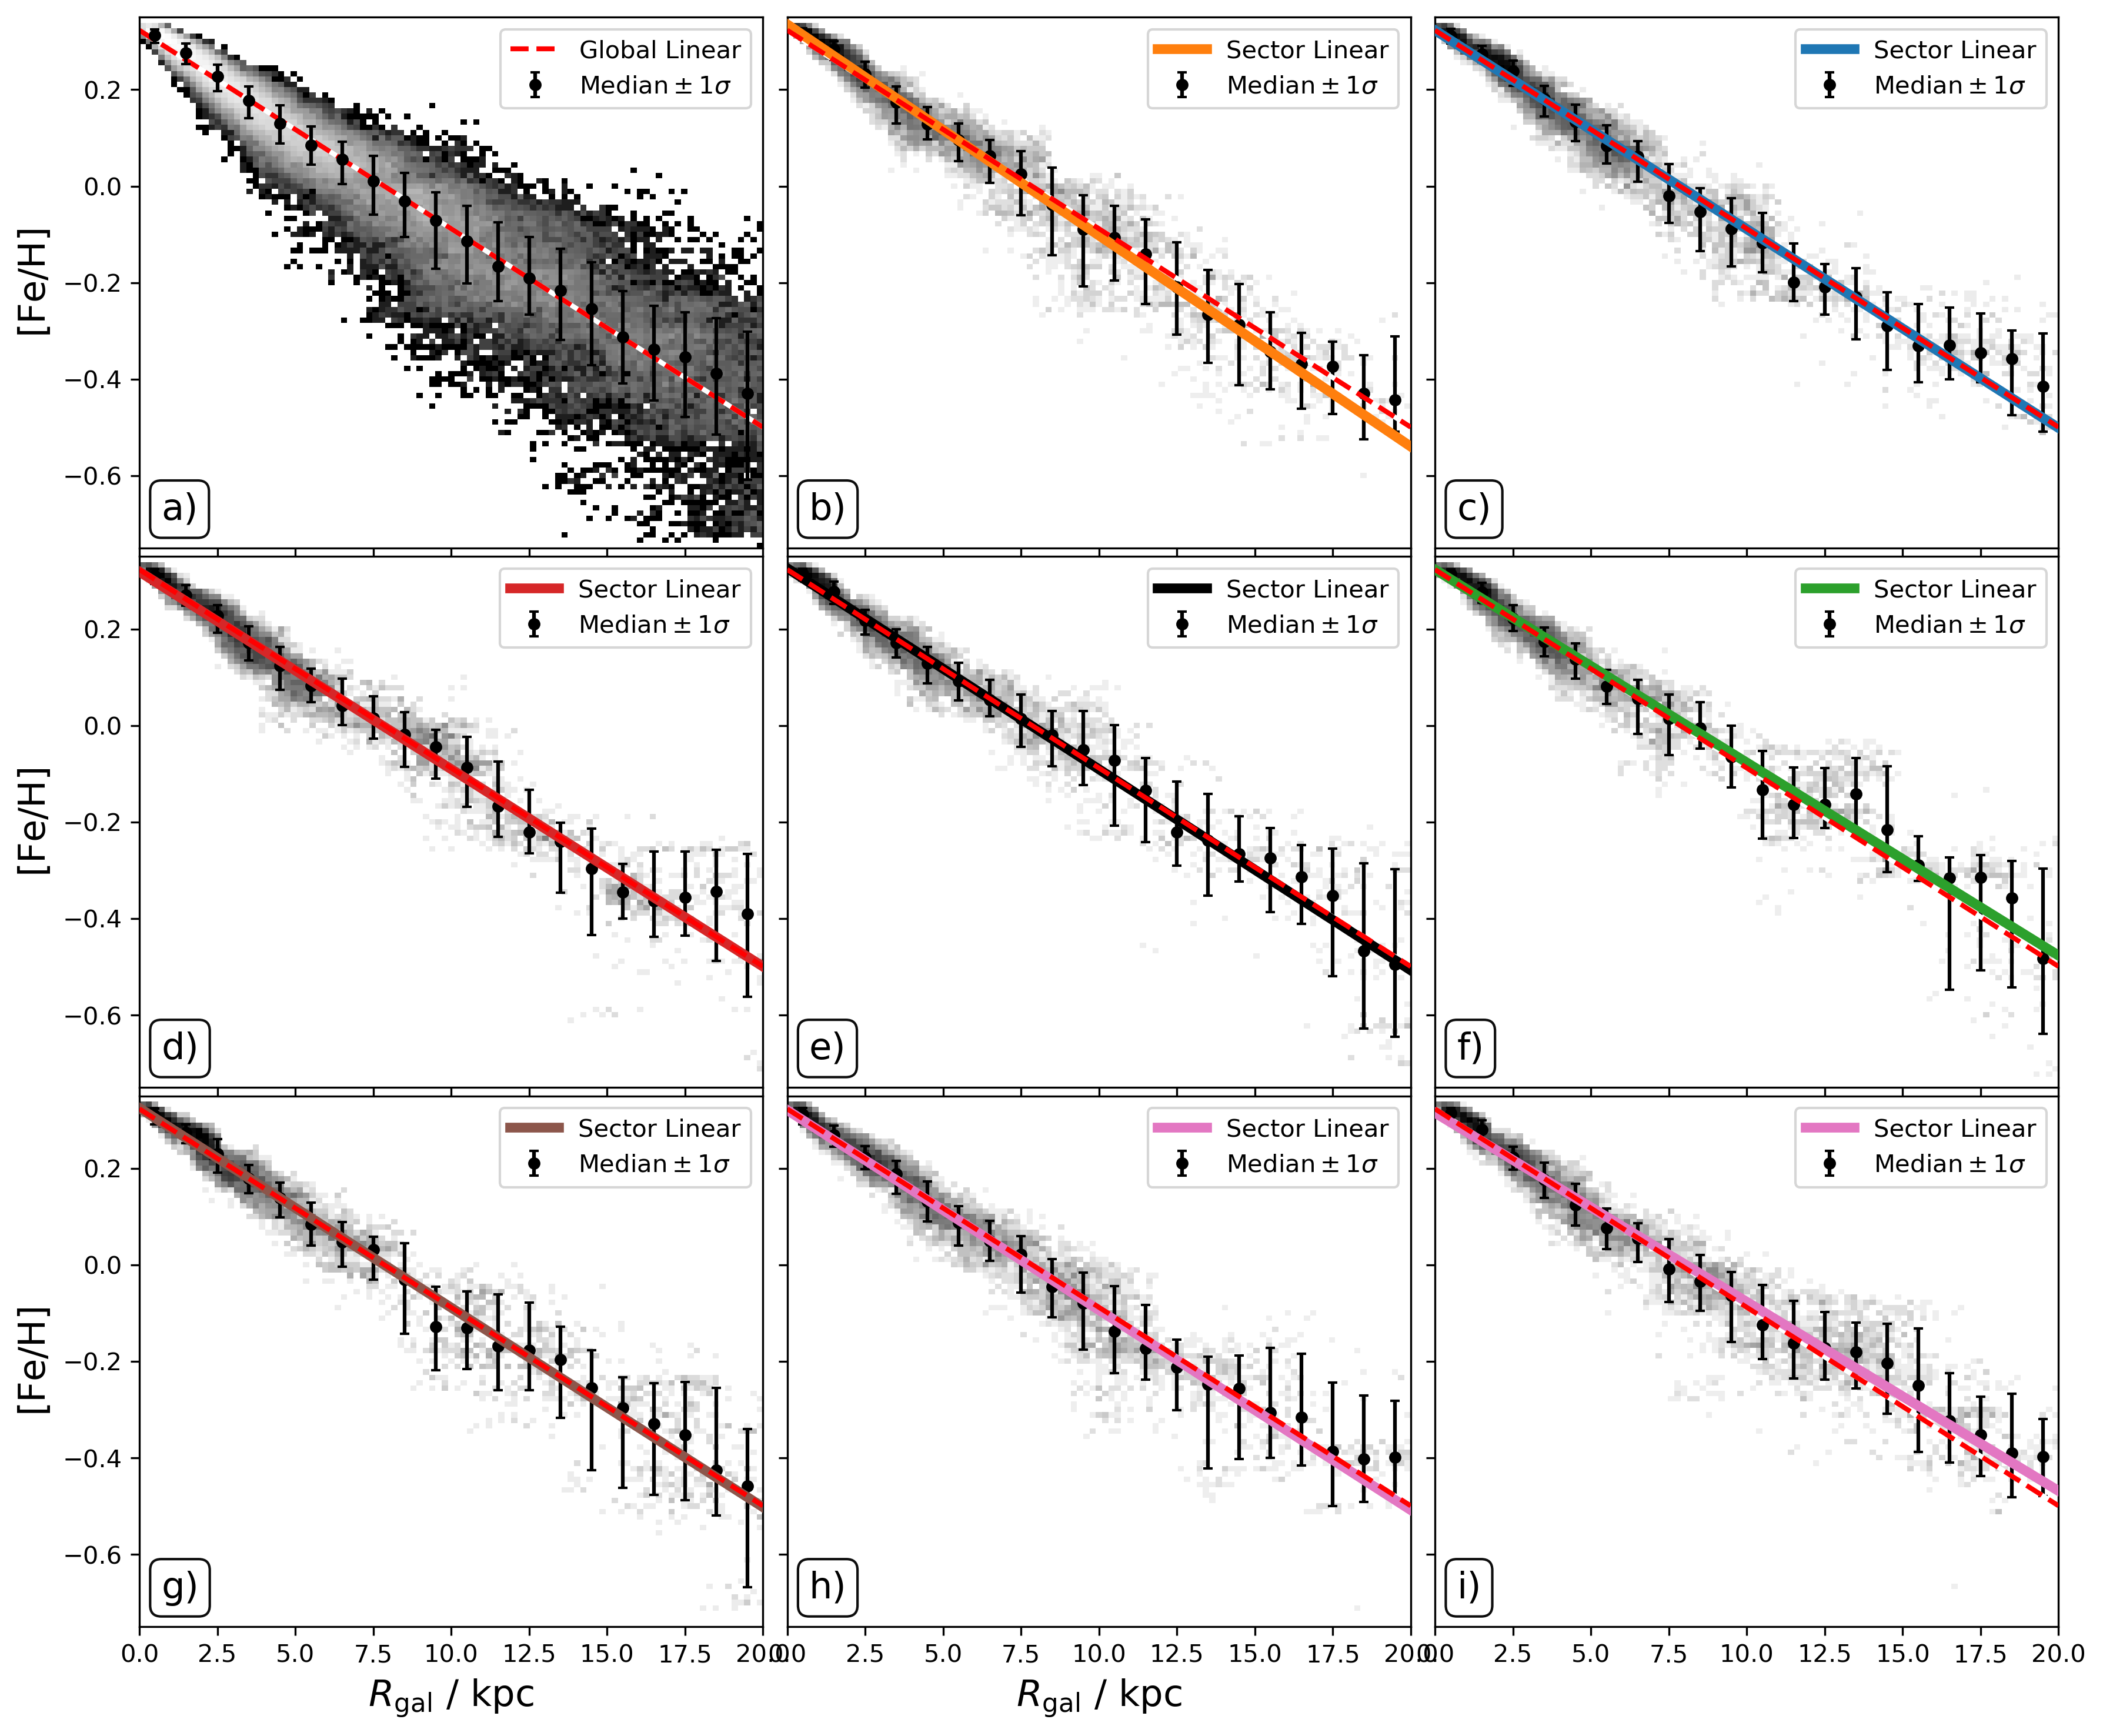
\includegraphics[width=\textwidth]{figures/linear_radial_metallicity_gradients_mw_in_angles.png}
    \caption{Density variation of the radial metallicity gradient $R-\mathrm{[Fe/H]}$ across full stellar disk (panel a) and 8 different sectors (same panel order as for Fig.~\ref{fig:radial_metallicity_gradients_mw_in_angles}). Linear radial metallicity gradients have been fit globally (red dashed line) and for each sector with colors following the same color code as in Fig.~\ref{fig:radial_metallicity_gradients_mw_in_angles}.}    \label{fig:linear_radial_metallicity_gradients_mw_in_angles}
\end{figure*}

\subsection{Coherence of the gradient with age}
\label{sec:coherence_age_radial_metallicity_gradients}

\SB{Do the same as Fig.~\ref{fig:radial_metallicity_gradients_mw_in_angles}, but with bins colored by median age.}

\SB{Global $R-\mathrm{[Fe/H]}$, then local for the 8 sectors of Fig.~\ref{fig:radial_metallicity_gradients_mw_in_angles}, plot both in 2x4 subpanels, and color-code the density plots by median deviation from this line with a seismic map.}

\begin{figure}
    \centering
    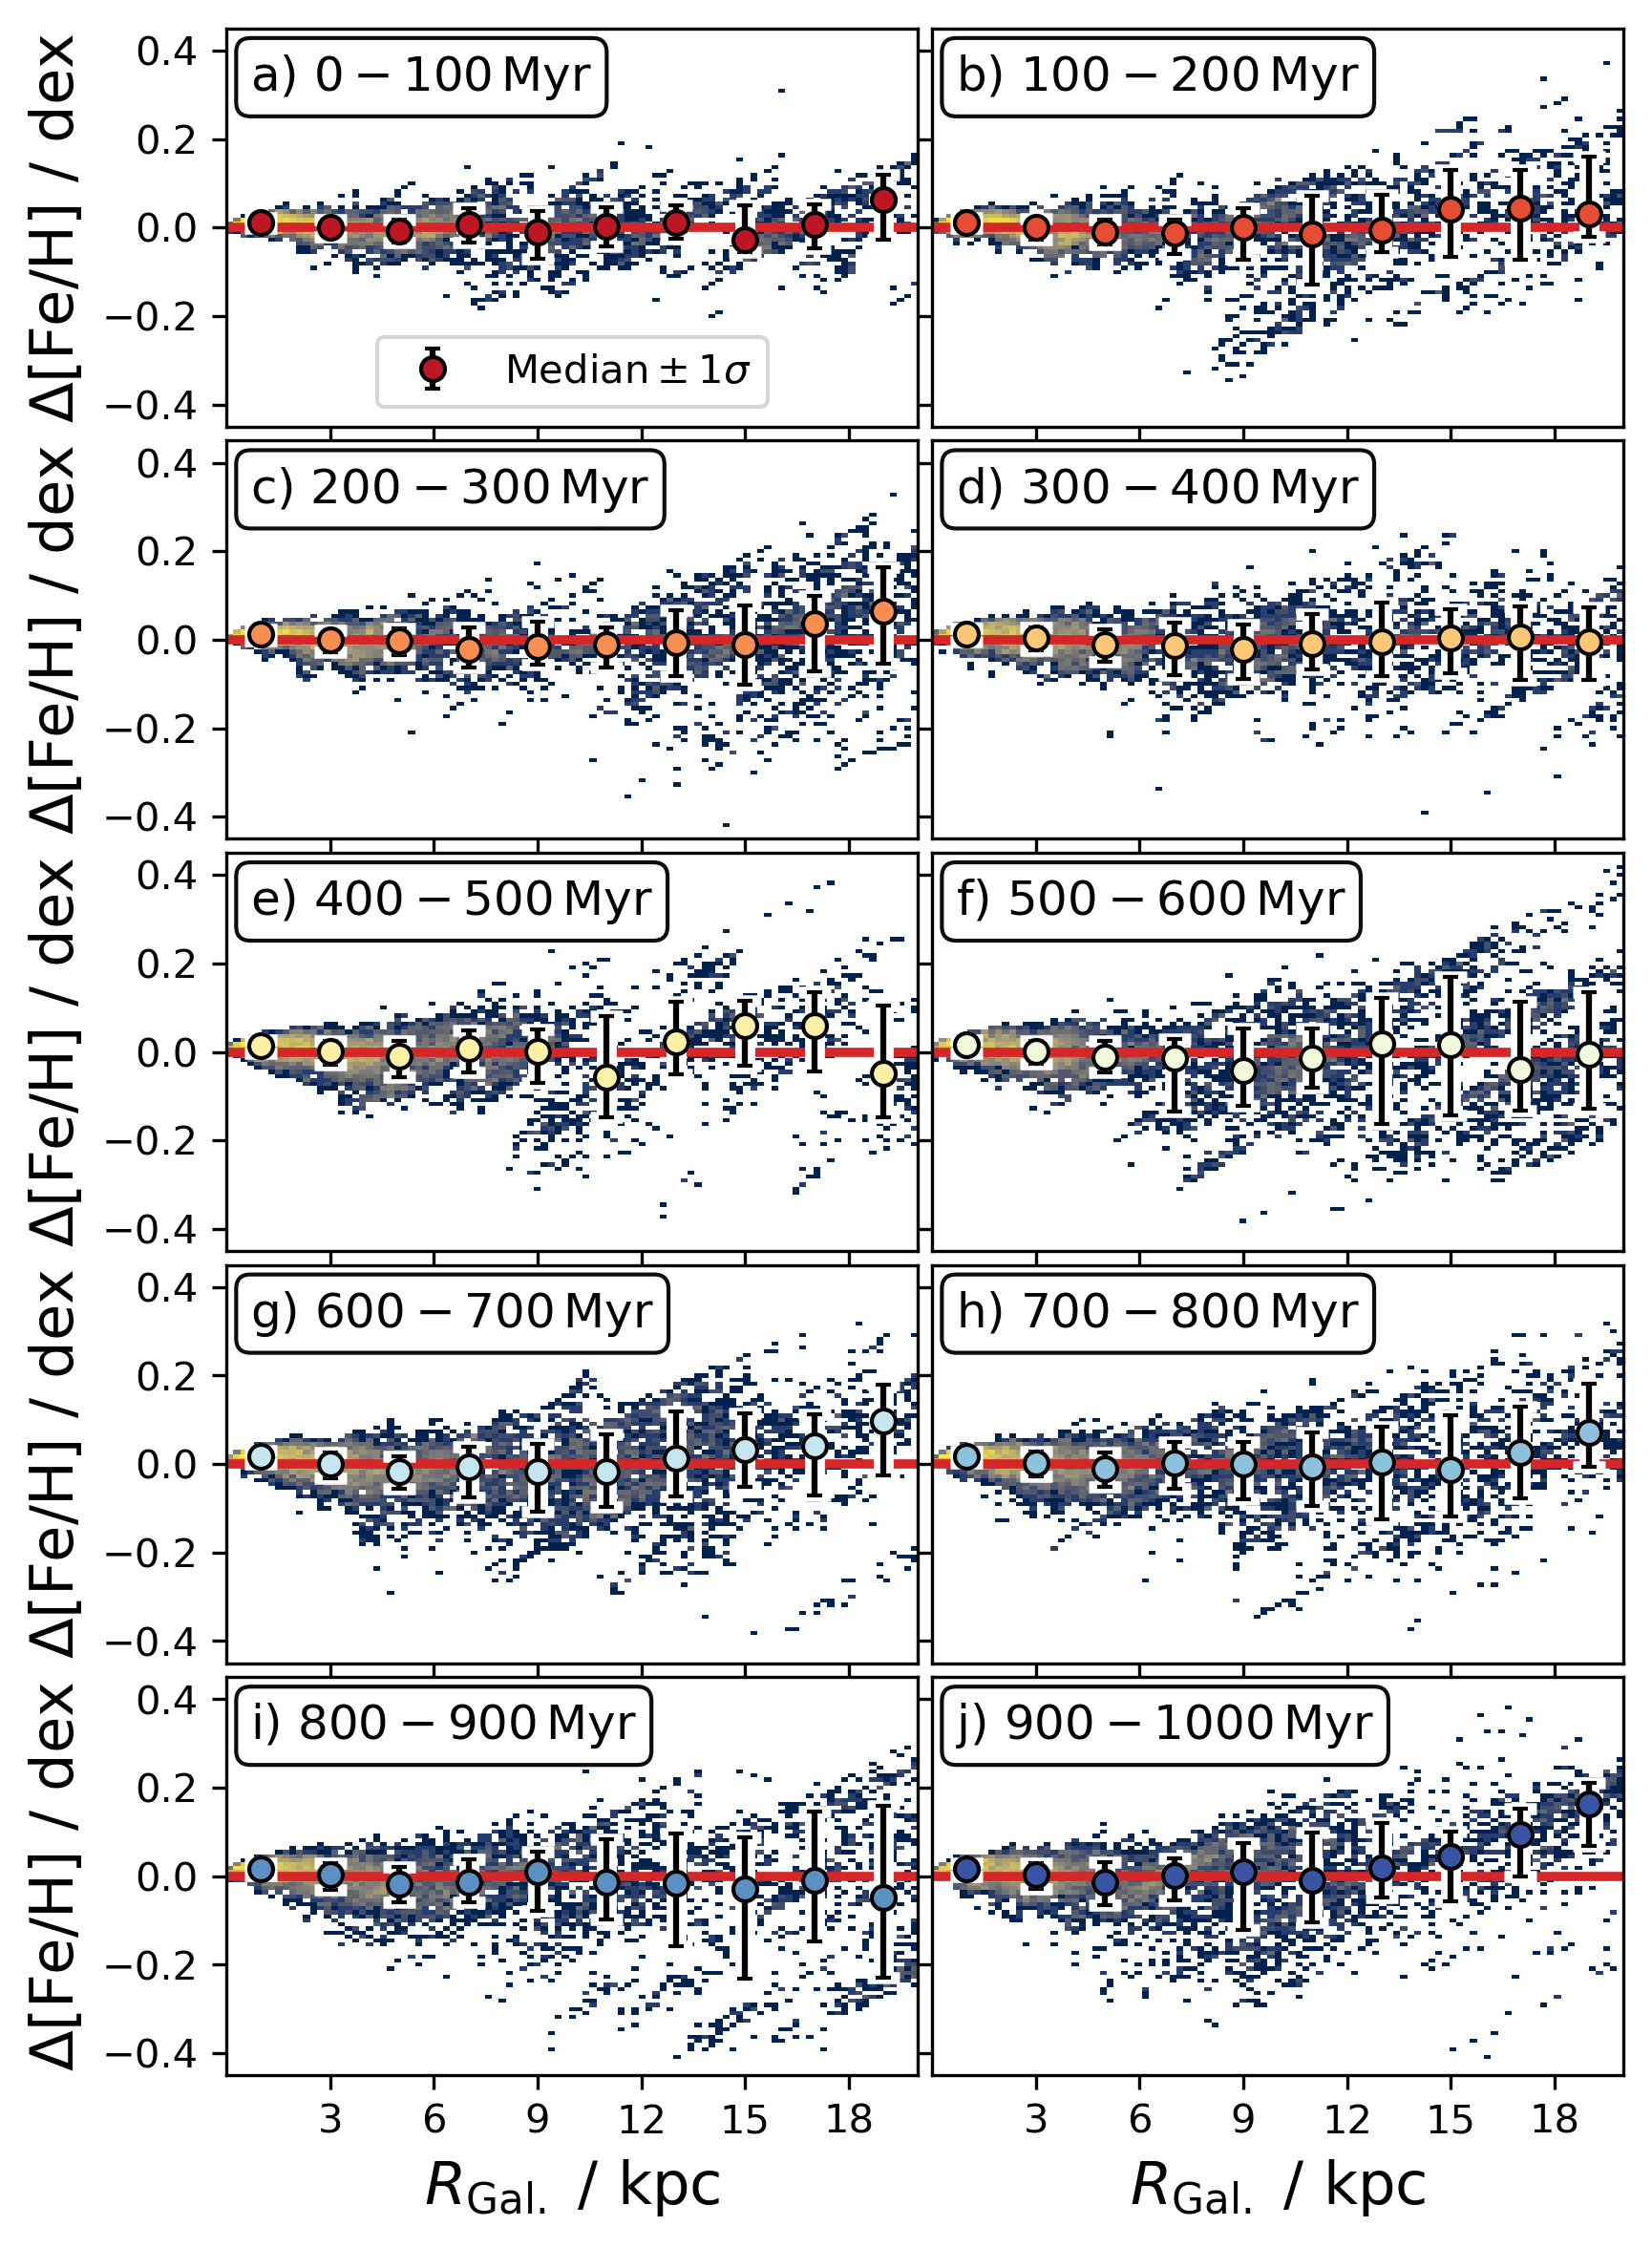
\includegraphics[width=\columnwidth]{figures/scatter_with_increasing_age.png}
    \caption{Density distribution and spread of [Fe/H] across different galactocentric radii with respect to a global linear radial metallicity gradient across different age ranges. Panels a-j) show young stars and exhibit a rather similar trend, whereas the scatter increases significantly for stars above $1\,\mathrm{Gyr}$ in panels panels k) and l).}
    \label{fig:scatter_with_increasing_age}
\end{figure}

\SB{see also scatter across age in Fig.~\ref{fig:scatter_with_increasing_age}}

The maximum scatter in radius bins varies between $0.073\,\mathrm{dex}$ and $0.195\,\mathrm{dex}$ across the $0..0.1..1.0\,\mathrm{Gyr}$ bins.%


Fig.~\ref{fig:linear_radial_metallicity_gradients_mw_in_angles}f shows impressively, that if you look at a rather narrow range of $R_\mathrm{gal}$, such as $7 < R_\mathrm{gal} < 13\,\mathrm{kpc}$, the radial metallicity gradient could actually look like it is damping towards larger radii. \SB{Is this possibly what is happening in local studies of our galaxy, where many researchers are actually fitting 2 linear gradients with a break radius?}

\SB{Actually one can see this effect even better in Fig.~\ref{fig:radial_metallicity_gradients_mw_in_angles}b,d,e,f,h and i!}

%%%%%%%%%%%%%%%%%%%%%%%%%%%%%%%%%%%%%%%%%%%%%%%%%%
\section{Discussion} \label{sec:discussion}

Comparison to \citet[][see their Fig. 10]{Minchev2014b}: They see significant decrease of stars towards larger radii (note to myself: their bins are not scatter, but number density in Fig. 10). How does this compare to our number densities?

\subsection{Linearity of the gradient} \label{sec:discussion_linearity}

\SB{How are the linear metallicity gradients usually measured? Any binning? If so, can we study what effect that has? How are uncertainties treated?}

To what extent is the radial metallicity gradient of young stars linear? Alternatively, would it be better described by two linear relations, with a break radius at corotation radius \citep[][and references therein]{Bresolin2012} or further out \citep{Donor2020} or a more sophisticated function \citep[see e.g.][]{Chiappini2001, Kubryk2015}? Investigating the gradient's form helps in understanding the galactic processes influencing metallicity at different radii \citep{Minchev2014b}.

\SB{"However, a simple, linear gradient may not be the better way to describe the distribution of the elements in the Galactic disk. From Cepheids, Andrievsky et al. (2002b), Pedicelli et al. (2009, 2010), and Genovali et al. (2013) found a steeper gradient in the very inner disk ($\leq 7\,\mathrm{kpc}$)." from \citet{Lemasle2013}}

\SB{"There are numerous abundance studies of open clusters from different groups: [...] They all reach the same conclusion: a linear gradient of approximately $-0.06\,\mathrm{dex/kpc}$ extending quite far into the outer disk, and a flattening at a level of $\mathrm{[Fe/H]} \approx -0.3\,\mathrm{dex}$, somewhere between 10 and 14 kpc." from \citet{Lemasle2013}.}

\SB{\citet{Lemasle2008} find $\mathrm{d[Fe/H]}/\mathrm{d}R = -0.050 \pm 0.008\,\mathrm{dex\,kpc^{-1}}$ in the 5-17 kpc range, but $\mathrm{d[Fe/H]}/\mathrm{d}R = -0.012 \pm 0.014\,\mathrm{dex\,kpc^{-1}}$ in a smaller 10-15 kpc range.}

\SB{Put some of these results into context of the Milky Way in Fig.~\ref{fig:radial_metallicity_gradients_mw_vs_nihao}.}

\begin{figure*}
    \centering
    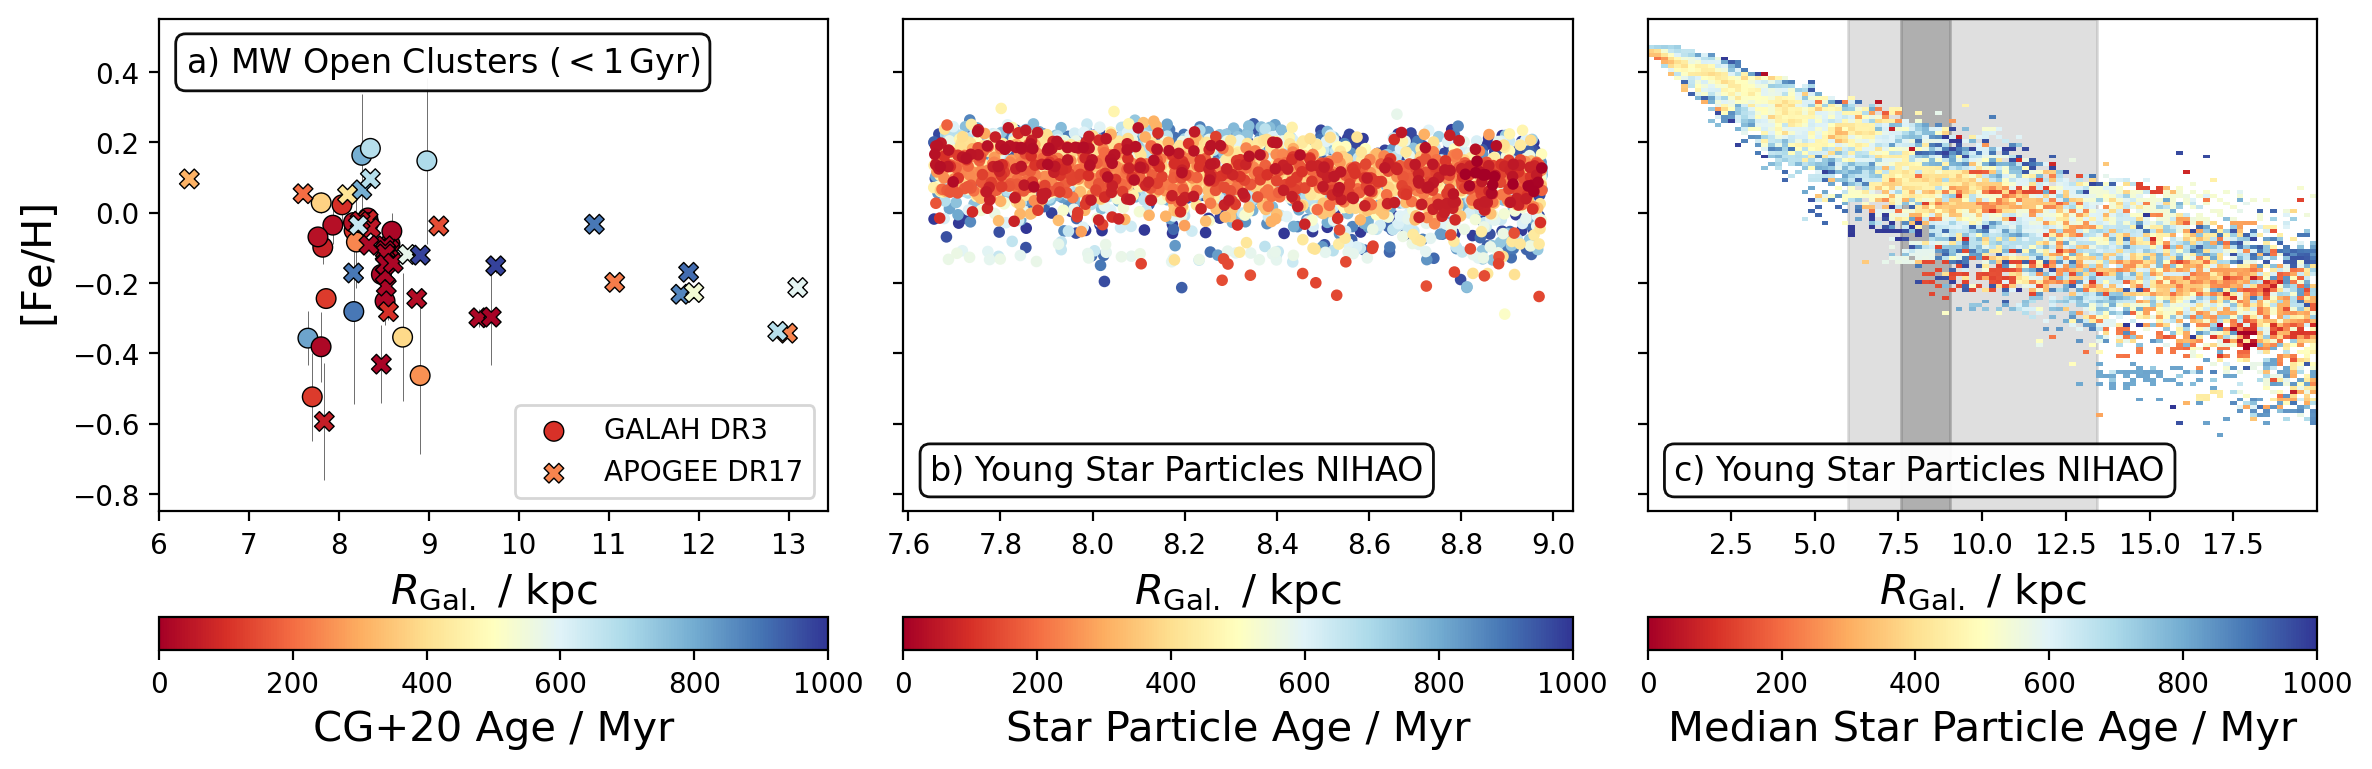
\includegraphics[width=\textwidth]{figures/radial_metallicity_gradients_mw_vs_nihao.png}
    \caption{Caption}
    \label{fig:radial_metallicity_gradients_mw_vs_nihao}
\end{figure*}

\subsection{Scatter in the gradient} \label{sec:discussion_scatter}

How much scatter in the radial metallicity gradient of young stars is expected based on simulations? Quantifying the scatter can provide insights into the effects of transient events like mergers, star formation bursts, and gas accretion.

\begin{itemize}
    \item 
\end{itemize}

\SB{Put some of these results into context of the Milky Way in Fig.~\ref{fig:overdensities_mw_vs_nihao}, e.g. \citet{Poggio2021} and \citet{Hackshaw2024}.}

\begin{figure*}
    \centering
    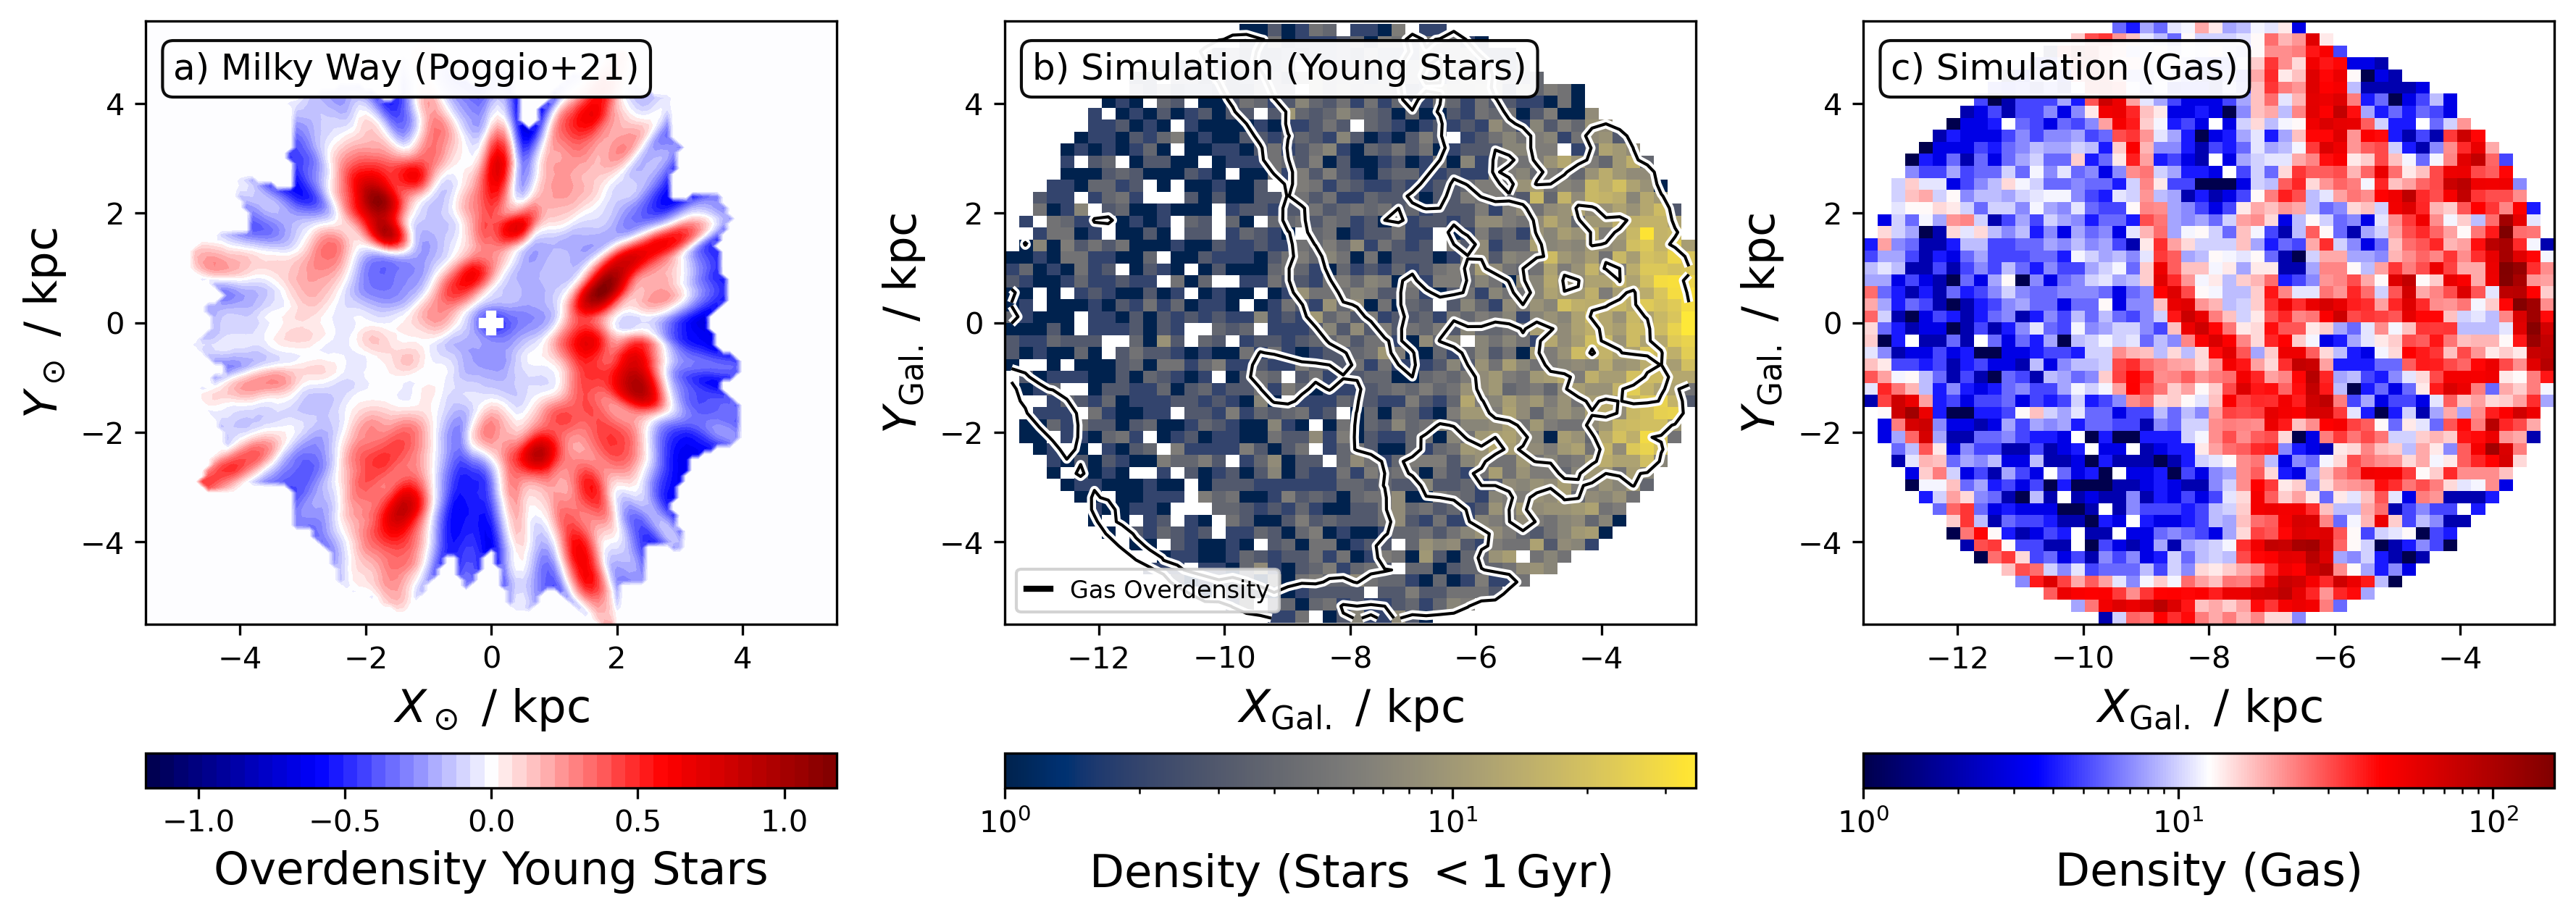
\includegraphics[width=\textwidth]{figures/overdensities_mw_vs_nihao.png}
    \caption{Caption}
    \label{fig:overdensities_mw_vs_nihao}
\end{figure*}

\subsection{Coherence of the gradient with position} \label{sec:discussion_coherence_position}

How significant is the change in the radial metallicity of young stars gradient as a function of position, both in terms of radial coverage and azimuth? Understanding these variations can reveal the underlying processes affecting metallicity distribution, such as spiral arm dynamics and bar-driven mixing \citep[see their Figs. 5-8][]{DiMatteo2013}.

\subsection{Coherence of the gradient with age} \label{sec:discussion_coherence_age}

Until what stellar age can stars be used as reliable tracers of the gas disk in simulations, in terms of both chemical composition and position? This question is pivotal for interpreting observed gradients across different ages \citep[e.g.][]{Willett2023} and comparing them with model predictions, particularly concerning the migration and heating of stellar populations \citep{Binney2008, Frankel2018}.

\subsection{Application of quadratic gradient function onto observations}

\begin{itemize}
    \item Can we apply our functional form onto MW data? e.g. \citet{Genovali2014}?
    \item Can we apply our functional form onto extragalactic data? e.g. \citet{Chen2023}?
\end{itemize}

%%%%%%%%%%%%%%%%%%%%%%%%%%%%%%%%%%%%%%%%%%%%%%%%%%
%%%%%%%%%%%%%%%%%%%%%%%%%%%%%%%%%%%%%%%%%%%%%%%%%%
\section{Conclusions}
\label{sec:conc}

\subsection{Main Take-Away}

\subsection{Future Research}

\begin{itemize}
    \item Can we say what the linear gradient and flattening part is for $R_\text{eff}$ for our NIHAO Milky Way analogue. Can we relate this to the MW effective radius and other galaxies?
\end{itemize}

\section*{Acknowledgements}

We acknowledge the traditional owners of the land on which the AAT and ANU stand, the Gamilaraay, the Ngunnawal and Ngambri people. We pay our respects to elders past, present, and emerging and are proud to continue their tradition of surveying the night sky in the Southern hemisphere.

This work was supported by the Australian Research Council Centre of Excellence for All Sky Astrophysics in 3 Dimensions (ASTRO 3D), through project number CE170100013. SB acknowledges support from the Australian Research Council under grant number DE240100150 which enabled SB to continue researching at the end of a fixed-term position and finalising this study. TB acknowledges funding from the Carl Zeiss Stiftung and support from the European Research Council under ERC-CoG grant CRAGSMAN-646955. We gratefully acknowledge the Gauss Centre for Supercomputing e.V. (\url{www.gaus s-centre.eu}) for funding this project by providing computing time on the GCS Supercomputer SuperMUC at Leibniz Supercomputing Centre (\url{www.lrz.de}). Simulations were partially computed with High Performance Computing resources at New York University, Abu Dhabi.

\section*{Facilities}

\textbf{AAT with 2df-HERMES at Siding Spring Observatory:} The GALAH Survey is based data acquired through the Australian Astronomical Observatory, under programs: A/2013B/13 (The GALAH pilot survey); A/2014A/25, A/2015A/19, A2017A/18 (The GALAH survey phase 1), A2018 A/18 (Open clusters with HERMES), A2019A/1 (Hierarchical star formation in Ori OB1), A2019A/15 (The GALAH survey phase 2), A/2015B/19, A/2016A/22, A/2016B/10, A/2017B/16, A/2018B/15 (The HERMES-TESS program), and A/2015A/3, A/2015B/1, A/2015B/19, A/2016A/22, A/2016B/12, A/2017A/14, (The HERMES K2-follow-up program). This paper includes data that has been provided by AAO Data Central (\url{datacentral.aao.gov.au}).

\textbf{\Gaia: } This work has made use of data from the European Space Agency (ESA) mission \Gaia (\url{http://www.cosmos.esa.int/gaia}), processed by the \Gaia Data Processing and Analysis Consortium (DPAC, \url{http://www.cosmos.esa.int/web/gaia/dpac/consortium}). Funding for the DPAC has been provided by national institutions, in particular the institutions participating in the \Gaia Multilateral Agreement. 

\textbf{Other facilities:} This publication makes use of data products from the Two Micron All Sky Survey \citep{Skrutskie2006} and the CDS VizieR catalogue access tool \citep{Vizier2000}.

\section*{Software}

The research for this publication was coded in \textsc{python} (version 3.7.4) and included its packages
\textsc{astropy} \citep[v. 3.2.2;][]{Robitaille2013,PriceWhelan2018},
\textsc{IPython} \citep[v. 7.8.0;][]{ipython},
\textsc{matplotlib} \citep[v. 3.1.3;][]{matplotlib},
\textsc{NumPy} \citep[v. 1.17.2;][]{numpy},
\textsc{pynbody} \citep[v. 1.1.0;][]{pynbody},
\textsc{scipy} \citep[v. 1.3.1;][]{Scipy},
\textsc{sklearn} \citep[v. 1.5.1][]{scikit-learn}
\textsc{statsmodels} \citep[v. 0.14.2][]{statsmodels}
We further made use of \textsc{topcat} \citep[version 4.7;][]{Taylor2005};

%%%%%%%%%%%%%%%%%%%%%%%%%%%%%%%%%%%%%%%%%%%%%%%%%
\section*{Data Availability}

All code and data to reproduce the analysis and figures can be accessed via \url{https://github.com/svenbuder/age_abundance_nihao_vs_galah}.

% The repository also includes the chemical and kinematic data of the simulated Milky Way analogue \texttt{g8.26e11} for last snapshot of the simulation for the observable footprint that were used for this study as well as the cleaned catalogue of GALAH DR3. All GALAH DR3 data is also published by \citet{Buder2021} and can be accessed publicly via \url{https://docs.datacentral.org.au/galah/dr3/overview/}. The full simulation data of \texttt{g8.26e11} can be obtained upon reasonable request from the authors. Currently the only limitation in making all data public is limited cloud space to host the data. We encourage interested readers to get in contact with the authors for full data access. Redshift zero snapshots from the original NIHAO-UHD simulations can be found here: \url{https://tobias-buck.de/\#sim_data}.

% If you are using either of these data to follow up on this research, remember to give appropriate credit to the researchers who created and curated either data set, that is, at least to \citet{Buder2021, Buder2022} and \citet{Buck2020b, Buck2021}.

%%%%%%%%%%%%%%%%%%%% REFERENCES %%%%%%%%%%%%%%%%%%

% The best way to enter references is to use BibTeX:
\bibliographystyle{mnras}
\bibliography{bib} % if your bibtex file is called example.bib

%%%%%%%%%%%%%%%%%%%%%%%%%%%%%%%%%%%%%%%%%%%%%%%%%%
%%%%%%%%%%%%%%%%% APPENDICES %%%%%%%%%%%%%%%%%%%%%

% \newpage
% \appendix


%%%%%%%%%%%%%%%%%%%%%%%%%%%%%%%%%%%%%%%%%%%%%%%%%%
% Don't change these lines
\bsp	% typesetting comment
\label{lastpage}
\end{document}